\documentclass[12pt,letterpaper]{article}

\usepackage{amsmath, amsthm}
\usepackage{graphicx,hyperref}
\usepackage{microtype, parskip}
\usepackage{natbib}
\usepackage{lineno}
\usepackage[font=small]{caption}
\usepackage{subcaption, multirow, morefloats}
\usepackage{subcaption, wrapfig}
\usepackage{titlesec}
\usepackage[nottoc,numbib]{tocbibind}
\usepackage{authblk, attrib, fullpage}
\usepackage{lineno}

\frenchspacing

\captionsetup[subfigure]{position = top, labelfont = bf, textfont = normalfont, singlelinecheck = off, justification = raggedright}

\renewcommand{\section}[1]{%
\bigskip
\begin{center}
\begin{Large}
\normalfont\scshape #1
\medskip
\end{Large}
\end{center}}

\renewcommand{\subsection}[1]{%
\bigskip
\begin{center}
\begin{large}
\normalfont\itshape #1
\end{large}
\end{center}}

\renewcommand{\subsubsection}[1]{%
\vspace{2ex}
\noindent
\textit{#1.}---}

\renewcommand{\tableofcontents}{}

\bibpunct{(}{)}{;}{a}{}{,}  % this is a citation format command for natbib

\title{How cryptic is cryptic diversity? Machine learning approaches to classifying morphological variation in the Pacific Pond Turtle (\textit{Emys marmorata})}
\author[1]{Peter D Smits}%\thanks{psmits@uchicago.edu}}
\author[1,2]{Kenneth D Angielczyk}%\thanks{kangielczyk@fieldmuseum.org}}
\author[3]{James F Parham}%\thanks{jparham@fullerton.edu}}
\affil[1]{Committee on Evolutionary Biology, University of Chicago}
\affil[2]{Integrative Research Center, Field Museum of Natural History}
\affil[3]{Department of Geological Sciences, California State University -- Fullerton}


\begin{document}
\maketitle
\noindent{\textbf{Corresponding author:} Peter D Smits, Committee on Evolutionary Biology, University of Chicago, 1025 E. 57th Street, Culver Hall 402, Chicago, IL, 60637, USA; E-mail: \href{mailto:psmits@uchicago.edu}{psmits@uchicago.edu}}

\linenumbers
\modulolinenumbers[2]

\begin{abstract}
  We investigate the morphometric identification of cryptic species using machine learning approaches by examining their implications for a recently proposed cryptic turtle species (\textit{Emys pallida}). We collected landmark-based morphometric data from 354 adult \textit{E. marmorata/``pallida''} museum specimens. We assigned a classification to each specimen for six different binning schemes based on geographic occurrence data recorded in museum collection archives. We used multiple machine learning methods, both unsupervised and supervised, to compare different classification hypotheses and asked whether it is possible to determine which amongst a set of classification hypotheses is best. In addition, we applied the above approach to a “clear-cut” example of seven unambiguously distinct species closely related to \textit{E. marmorata}. The results of this study indicate that there is no clear grouping of \textit{E. marmorata/``pallida''} based on plastron shape. In contrast, the analysis of the ``clear-cut'' example demonstrates a near perfect classification, which demonstrates that the methods can recover correct results when an appropriate signal exists. Explanations for the lack of grouping in \textit{E. marmorata} include that possibility that genetic differentiation is not associated with plastron shape variation below the species level and/or that local selective pressures (e.g., from hydrological regime) overwhelm morphological differentiation. A reconsideration of the methods used to delimit \textit{E. ``pallida,''} the lack of barriers to gene flow, the strong evidence for widespread admixture between lineages, and the fact that plastron shape can be used to differentiate other emydine species suggest that its lack of diagnosability most likely reflects the non-distinctiveness of this proposed taxon.
\end{abstract}

\section{Introduction}

% cryptic diversity
%   most species are still deliminated solely based on morphology
Molecular systematics has repeatedly demonstrated the existence of cryptic species that can only be diagnosed using genetic data \citep{Stuart2006,Bickford2007,SchlickSteiner2007,Pfenninger2007,Clare2011,Funk2012}. In attempts to streamline the documentation of biodiversity, several methods of species delimitation that rely almost entirely on genetic data have recently been proposed \citep{Pons2006,Carstens2010,Hausdorf2010,O'Meara2010,Yang2010b,Huelsenbeck2011b}. Although strong caveats on the utility of these methods have been raised \citep{Bauer2000,Carstens2013}, they are nevertheless being used to name species \citep{Leache2010,Spinks2014}.

The majority of extant taxa, and almost all extinct taxa, are delimited by morphology alone. This disjunction complicates interpretations of variation and diversity in deep time, as apparent morphological stasis may not reflect the true underlying diversity \citep{Eldredge1972,Gould1977a,Hunt2008,VanBocxlaer2013}. Similarly, for many museum specimens of extant taxa (e.g. those preserved in formalin), it is difficult to acquire the genetic data needed for non-morphological species delimitation methods.

These considerations have sparked interest in whether geometric morphometric analyses can capture fine-scale variation that can be used for identifying cryptic species. This would make the task of idetifying and maintaining endagered or conserved groups much easier and could contribute to improved classifications of extinct taxa and populations. Most such studies focus on using morphometrics to discover differences between taxa that were identified by other means \citep{Polly2003,Zelditch2004,Gaubert2005b,Gunduz2007,Polly2007a,Demandt2009}. Additionally, there has been work on automated taxon identification and classification of taxa into groups \citep{Baylac2003,Dobigny2003,MacLeod2007,VandenBrink2011}. 

Here, we investigate the morphometric identification of cryptic species using machine learning approaches. In particular, we ask whether it is possible to determine which amongst a set of classification hypotheses is best and examine the implications of the results for a recently proposed set of cryptic turtle species.

% past work on automatic taxon identification and older approaches to classifying taxa
% why use machine learning methods
\subsection{Background and study system}
Machine learning is an extension of known statistical methodology \citep{Hastie2009} that emphasizes high predictive accuracy and generality at the expense of the interpretability of individual parameters. The basic statistical mechanics are supplemented by randomization, sorting, and partitioning algorithms, along with the maximization or minimization of summary statistics, in order to best estimate a general model for all data, both sampled and unsampled \citep{Hastie2009}. Machine learning approaches have found use in medical research, epidemiology, economics and automated image identification such as handwritten zip codes \citep{Hastie2009}. The two major classes of machine learning methods are unsupervised and supervised learning. Unsupervised learning methods are used with unlabeled data where the underlying structure is estimated, and they are analogous to clustering and density estimation methods \citep{Kaufman1990}. Supervised learning methods are used with labeled data where the final output of data is known and the rules for going from input to output are inferred. These are analogous to classification and regression models \citep{Breiman1984}. Our application of the approaches used in this study illustrates only a sampling of the various methods available for clustering observations and fitting classification models. 

Geometric morphometric approaches to identifying differences in morphological variation between different classes, including cryptic species, mostly have used methods like linear discriminate analysis and canonical variates analysis \citep{Polly2003,Zelditch2004,Gaubert2005b,Gunduz2007,Polly2007a,Francoy2009,Sztencel-Jabonka2009,MitrovskiBogdanovic2013}. Because of their similarity to multivariate approaches like principle components analysis (PCA), these methods are comparatively straightforward ways of understanding the differences in morphology between classes. They also benefit from producing results that can be easily visualized, which aids in the interpretation and presentation of data and results. Most previous morphometric studies did not assess which amongst a set of alternative classification hypotheses was optimal. For example, studies such as those of \citet{Caumul2005a} and \citet{Polly2007a} focused on comparing different aspects of morphology and their fidelity to a classification scheme instead of comparing the fidelity of one aspect of morphology to multiple classification schemes. In this context, the study of \citet{Cardini2009a} is noteworthy because they compared morphological variation in marmots at the population, regional, and species level and determined the fidelity of shape to divisions at each of these levels.

Here, we used multiple machine learning methods, both unsupervised and supervised, to compare different classification hypotheses. These methods provide different advantages for understanding how to classify taxa, as well as the accuracy of the resulting classifications. Although machine learning methods such as neural networks have been applied to studying shape variation \citep{Baylac2003,Dobigny2003,MacLeod2007,VandenBrink2011}, including in the context of automated taxon identification and classification of groups, the number of cases remains limited. In the current study, we not only consider pure classification accuracy but also use a statistic of classification strength that reflects the rate at which taxa are both accurately and inaccurately classified. 


We analyzed the problem of whether there are distinct subspecies or cryptic species within the western pond turtle, \textit{Emys marmorata} \citep{Baird1852} (formerly \emph{Clemmys marmorata}; see \citealp{Feldman2002}). \textit{Emys marmorata} is distributed from northern Washington State, USA to Baja California, Mexico. Traditionally, \textit{E. marmorata} was classified into two named subspecies: the northern \textit{E. marmorata marmorata} and the southern \textit{Emys marmorata pallida} \citep{Seeliger1945}, with a central Californian intergrade zone in between. \textit{Emys marmorata marmorata} is differentiated from \textit{E. marmorata pallida} by the presence of a pair of triangular inguinal scales and darker neck markings. The triangular inguinal plates can sometimes be present in \textit{E. marmorata pallida} although they are considerably smaller. \citet{Seeliger1945} did not formally include the Baja California populations of \textit{E. marmorata} in either taxon, implying the existence of a third distinct but unnamed subspecies.

Previous work on morphological variation in \textit{E. marmorata} has focused primarily on differentiation between populations over a portion of the species' total range \citep{Lubcke2007,Germano2008,Germano2009,Bury2010}; comparatively few studies have included specimens from across the entire range \citep{Holland1992}. Most of these studies considered how local biotic and abiotic factors may contribute to differences in carapace length and found that size can vary greatly between different populations \citep{Lubcke2007,Germano2008,Germano2009}. There also has been interest in size-based sexual dimorphism in \textit{E. marmorata} \citep{Holland1992,Lubcke2007,Germano2009}, with males being on average larger than females based on total carapace length and other linear measurements. However, the quality of size as a classifier of sex can vary greatly between populations \citep{Holland1992} because of the magnitude of size differences among populations \citep{Lubcke2007,Germano2009}. However, the effect of sexual dimorphism on shape, \textit{sensu} \citet{Kendall1977a}, has not been assessed \citep{Holland1992,Lubcke2007,Germano2008}.

Of particular importance in the context of cryptic diversity in \textit{E. marmorata} is the morphometric analysis of carapace shape carried out by \citet{Holland1992}, who compared populations of \textit{E. marmorata} from three areas of its range. This study concluded that geographic distance was a poor indicator of mophological differentiation, and instead hypothesized that geographic features such as breaks between different drainage basis are probably more important barriers to dispersal and interbreeding. Additionally, \citep{Holland1992} suggested that morphological differences were more pronounced as the magnitude of barriers and distance increased, but this variation required many variables to adequately capture, implying only very subtle morphological differentiation between putatively distinct populations. Finally, Holland concluded that \textit{E. marmorata} is best classified as three distinct species: a northern species, souther species, and a Columbia Basin species. This classification is similar to that of \citet{Seeliger1945}, except elevated to the species level and without recognition of a distinct Baja species. 

More recently, the phylogeography of \textit{E. marmorata} and the possibility of cryptic diversity was investigated using molecular data \citep{Spinks2005,Spinks2010,Spinks2014}. Based on mitochondrial DNA, \citet{Spinks2005} recognized four subclades within \textit{E. marmorata}, a northern clade, a San Joaquin Valley clade, a Santa Barbara clade, and a southern clade. Analyses with nuclear DNA \citep{Spinks2010} and single-nucleotide polymorphism (SNP) data suggest a primarily north--south division in \textit{E. marmorata}, although the dataset differed from that of \citet{Spinks2005} in the location of this break point. These studies discussed the potential taxonomic implications of their results, with \citet{Spinks2014} going so far as to strongly advocate for the recognition of at least two species (\emph{E. marmorata} and \emph{E. pallida}), and a possible third based on populations in Baja California. However, they did not discuss in detail the morphological characters that would help to diagnose these species beyond those specified by \citet{Seeliger1945}. Given that these characters are somewhat variable within the proposed species, and that \citet{Holland1992} described shell shape variation that might be consistent with this taxonomy, a geometric morphometric analysis of shell shape might provide a reliable way to diagnose groups (whether species or subspecies) within \textit{E. marmorata}.

In this study, we attempt to estimate the best classification scheme of \textit{E. marmorata} based on variation in plastron (ventral shell) shape in order to determine whether this character is consistent with any of the past divisions based on other morphological features or molecular data. We are particularly interested in whether any aspect of plastron shape can be used to reliably diagnose \citet{Spinks2014} proposed species, and if so, the nature of that shape variation.

Because of unclear geographic boundaries between subgroups of \textit{E. marmorata}, we compare multiple hypotheses of morphologically-- and molecularly--based classification. We hypothesize that if morphological variation corresponds to class assignment, it should be possible to determine the best classification hypothesis of \textit{E. marmorata} from amongst multiple candidate hypotheses. However, if morphological variation does not correspond to any of the standing hypothesis, then supervised learning model generalization performance will be poor.


\section{Materials and Methods}
\subsection{Specimens, sampling, morphometrics}
We collected landmark-based morphometric data from 354 adult \textit{E. marmorata} museum specimens. These specimens are a subset of those included in \citet{Angielczyk2007}, \citet{Angielczyk2011}, and \citet{Angielczyk2013a}, essentially representing the adult individuals included in those papers. We chose to focus on adults because significant changes in plastron shape occur over the course of ontogeny in \textit{E. marmorata} and other emydines \citep{Angielczyk2013a}.

We assigned a classification to each specimen for the different binning schemes based on geographic occurrence data recorded in museum collection archives. When precise latitude and longitude information were not available we estimated them from locality information. Because \citet{Spinks2005}, \citet{Spinks2010}, and \citet{Spinks2014} did not use vouchered specimens we were not able to directly sample individuals in their studies. Therefore our specimen classifications were based solely on the geographic information, not explicit assignment using molecular data. Because the exact barriers between different biogeographic regions are unknown and unclear, we represented each hypothesis with two schemes for a total of six different schemes. The schemes differed based on where geographic boundaries were assigned. This changes the classification of certain individuals near the boundaries between groups, providing a test of the robustness of the classification schemes.

\begin{figure}[ht]
  \centering
  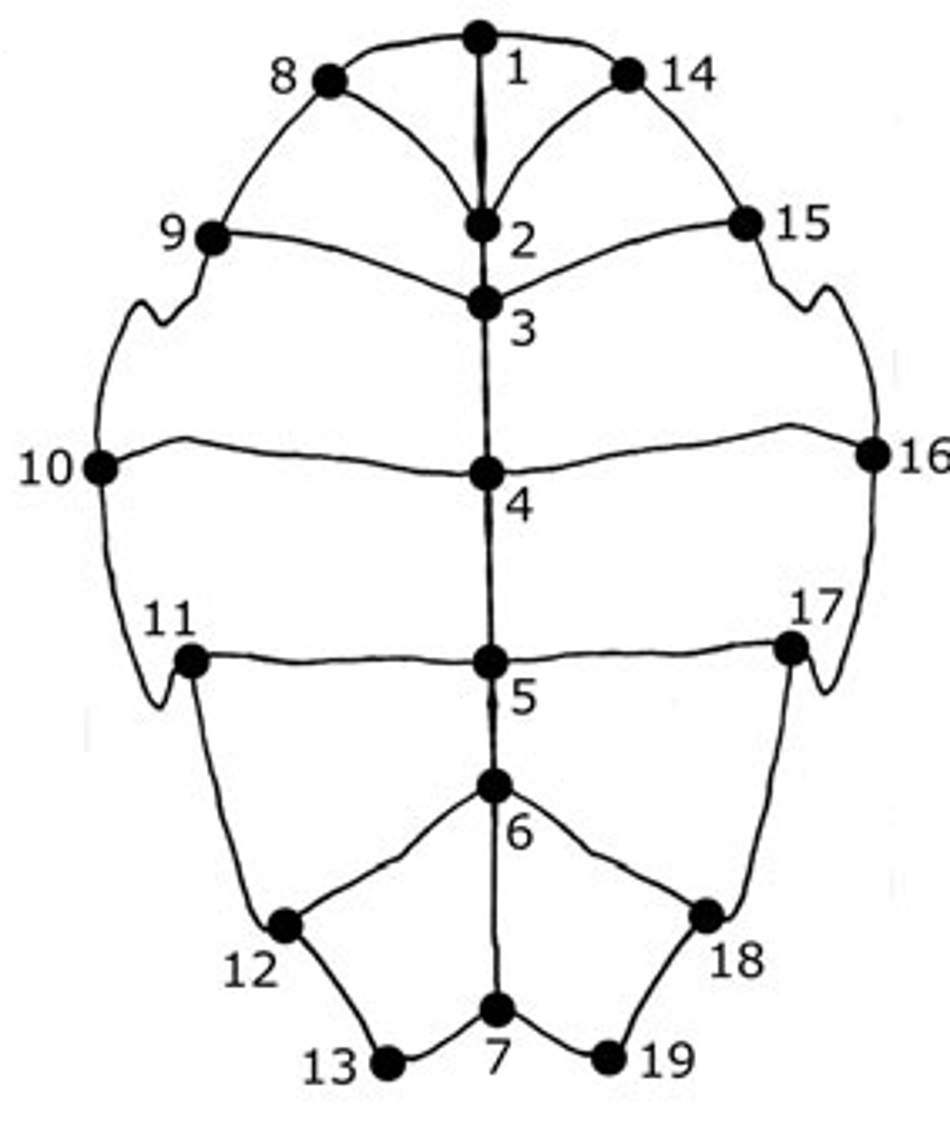
\includegraphics[height = 0.5\textheight, width = \textwidth, keepaspectratio = true]{figure/plastra}
  \caption{Depiction of general plastral shape of \textit{E. marmorata} and position of the 19 landmark used in this study. Anterior is towards the top of the figure.}
  \label{fig:plastra}
\end{figure}

Following previous work on plastron variation \citep{Angielczyk2007,Angielczyk2011,Angielczyk2013a}, we used TpsDig 2.04 \citep{Rohlf2005} to digitize 19 landmarks (Fig. \ref{fig:plastra}). Seventeen of the landmarks are at the endpoints or intersection of the keratinous plastral scutes that cover the platron. Twelve of the landmarks were symmetrical across the axis of symmetry and, in order to prevent issues related to degrees of freedom and other similar concerns \citep{Klingenberg2002}, we reflected these landmarks across the axis of symmetry (i.e. midline) prior to analysis and used the average position of each symmetrical pair. In cases where damage or incompleteness prevented symmetric landmarks from being determined, we used only the single member of the pair. We conducted all subsequent analyses on the resulting ``half'' plastra. We superimposed the plastral landmark configurations using generalized Procrustes analysis \citep{Dryden1998a}, after which, we calculated the principal components (PC) of shape using the \texttt{shapes} package for R \citep{2013,Dryden2013}.


\subsection{Machine learning analyses}
\subsubsection{Unsupervised learning}
In order to preserve the relationship between all landmark configurations in shape space, we measured the dissimilarity between observations using Kendall's Riemannian shape distance or \(\rho\) \citep{Kendall1984a,Dryden1998a}. We chose this metric because shape space, or the set of all possible shape configurations following Procrustes superimposition, is a Riemannian manifold and thus non-Euclidean \citep{Dryden1998a}. \(\rho\) varies between 0 and \(\pi / 2\) when there is no reflection invariance, which should not be a concern in the case of the half plastral landmark configurations used in the study.

We divisively clustered the shape dissimilarity matrix using partitioning around mediods clustering (PAM), a method similar to \textit{k}-means clustering except that instead of minimizing the sum of squared Euclidean distances between observations and centroids, the sum of squared dissimilarities between observations and mediods is minimized \citep{Kaufman1990}. Because the optimal number of clusters of shape configurations in the study was unknown, being possibly three, four, or some other value, we estimated clustering solutions in which the number of clusters varied between one and eight. We compared clustering solutions using the gap statistic, which is a measure of goodness of clustering \citep{Tibshirani2001a}.

%The gap statistic is defined
%\[Gap_{n}(k) = E^{*}_{n}[\log(W_{k})] - \log(W_{k})\] 
%where \(W_{k}\) is
%\[W_{k} = \sum^{k}_{r = 1}{\frac{1}{2n_{r}} (\sum_{i,i' \in C_{r}} d_{ii'})}\].
%\(d_{ii'}\) is the dispersion of the clustering solution or the sum of the pairwise dissimilarities between observations in each cluster and their respective mediods (\(C\)) for all clusters \(r\). This value is averaged and compared to the expected dispersion (\(E^{*}_{n}\)) of a sample \(n\) from a reference distribution. In this case, the reference distribution was estimated from 500 resamples.

We conducted this analysis using the \texttt{cluster} package for R \citep{Maechler2013}.

\subsubsection{Supervised learning}
We used three different supervised learning, or classification, approaches: linear discriminate analysis, multinomial logistic regression, and random forests. Linear discriminate analysis, also known as canonical variate analysis, is commonly used in studies of geometric morphometric data \citep{Zelditch2004,Mitteroecker2011}. The other two methods, however, are not. In all cases, the optimal number of PCs used as predictors was chosen via maximum within-sample AUC value, explained below.

Linear discriminate analysis (LDA) attempts to find a linear combination of predictors that best model two or more classes. LDA is very similar to PCA except that instead of finding the linear combination of features that maximize the amount of explained variance in the data, LDA maximizes the differences between classes. The results of this analysis produces a transformation matrix by which the original features can be transformed to reflect the best discrimination between the classes. In this study, we applied LDA to the eigenscores from a subset of the total number of PCs, ranging from two to six in increasing order of complexity. In total, this produced nine different LDA scaling matrices. 

Multinomial logistic regression is an extension of logistic regression, where instead of a binary response there are three or more response classes \citep{Venables2002a}. Similar to the odds ratios calculated from the coefficients of a logistic regression, the relative risk of a classification can be determined from the coefficients of the model.

Random forest models are an extension of classification and regression trees (CART) \citep{Breiman1984,Breiman2001}. The goal of CARTs is to use a series of different features (i.e. predictors) to estimate the class of an observation. In top-down induction of decision trees for each member of a given set of predictor variables, attribute value tests are used to estimate the differences between classes. This process, called recursive partitioning, is then repeated on each subset. The recursion continues until the resulting observations all share the same class or no more meaningful partitions are possible. The resulting model is a tree structure by which observations are classified at each intersection via the estimated cutoff points from the attribute tests made during model fitting. % figure to help explain the ``tests''

In a random forest model, many CARTs are built from a random subsample of both the features and the observations (specimens). This process is then repeated many times and the parameters of the final model are chosen as the mode of estimates from the distribution of CARTs \citep{Breiman2001}. In addition to classifying the observations, this procedure allows for the features to be ranked in order of importance. This is a generally useful property for studies in which the goal is to describe and model the differences between classes and the relative importance of different predictors. 

In this analysis, we used 1000 subtrees to estimate the random forest model parameters. We estimated the best set of predictors necessary for each classification scheme using a recursive feature selection algorithm, and we chose the optimal number of PCs to include based on the AUC of the model. Following the backwards selection algorithm implemented in \texttt{caret} \citep{KuhnMAN2013}, the maximum number of features were included in the initial model, their importance ranked, and the AUC of the model calculated. The lowest ranked feature was then removed, and the AUC of the model recalculated. This was repeated until only one feature, remained. Because PCs were kept in order of importance and not in relation to the amount of variance each PC described, the PCs are not included in the order of ascending eigenvalue.

In classification studies, such as this one, a common metric of performance is area under the receiver operating characteristic curve (AUC). AUC is an estimate of the relationship between the false positive and true positive rates, as opposed to just the true positive rate (accuracy). This relationship is especially useful in cases such as this study where misclassification needs to be minimized just as much as an accurate classification must be obtained. AUC ranges between 0.5 and 1, with 0.5 indicating classification no better than random and 1 indicating perfect classification \citep{Hastie2009}.

The standard AUC calculation is defined for binary classifications, however in our application there are multiple categories. The alternative calculation that we used follows an all-against-one strategy where the individual AUC values for each class versus all others are averaged to produce a multiclass AUC \citep{Hand2001}. To estimate confidence intervals on the out-of-sample AUC values, we performed a nonparametric bootstrap in which the true and estimated classifications were resampled with replacement. This was done 1000 times.

The ultimate measure of model fit is accurately predicting the values of unobserved samples \citep{Hastie2009,Kuhn2013}. Within-sample performance is inherently biased upwards, so model evaluation requires overcoming this bias. With very large sample sizes, as in this study, part of the sample can be used as the ``training set'' and the remainder acts as the ``testing set.'' The former is used for fitting the model where as the later is used for measuring model performance, a process called model generalization. In this analysis, we used 75\% of samples as the training set while the remaining 25\% were used as the testing set.

It is common for some out of sample observations to be misclassified. This misclassification may be due to the model not accurately representing shape variance, systematic differences between the training and test sets, or systematic differences between the accurately and inaccurately classified samples. Testing and training sets are determined completely at random within each class and with respect to shape. Results were not effected by the individual specimen class assignments to the testing or training sets.

To determine if there were systematic differences in plastron shape between the correctly and incorrectly classified samples, we used a permutation test to estimate if the dissimilarity between the correctly and incorrectly classified individuals was significantly greater than random. The group labels were permuted 1000 times and the distance between the new centroids was calculated. The number of permutations less than the empirical difference divided by 1000 gives a \textit{p}-value for the test. Significant results indicate that correctly and incorrectly classified specimens are systematically different. This was done only for classes where there were 10 or more observations.

\subsection{Comparison with clear-cut example}
In addition to the above analysis of classification schemes of \textit{E. marmorata/pallida}, we applied the above approach to a selection of seven morphologically distinct emydine species. This additional analysis was done in order to confirm the efficacy of our supervised learning approach. The seven species analyzed were \textit{Emys blandigii}, \textit{Terrapene coahuila}, \textit{Clemmys guttata}, \textit{Glyptemys insculpta}, \textit{Glyptemys muhlenbergii}, \textit{Emys orbicularis}, and \textit{Terrapene ornata} with a total of 578 specimens analyzed in total. Again, these data were a subset of those used in \citet{Angielczyk2011} and \citet{Angielczyk2013a}.

As with the \textit{E. marmorata/pallida} analysis, we analyzed plastron shape variation. The support for a seven category classification scheme was evaluated using random forest, linear discriminate analysis, and multinomial logistic regression where the number of PCs used as predictors ranged from two to 11. Data were split into training and testing sets and model performance for both sets was evaluated using the AUC metric.


\section{Results}

\subsection{Unsupervised learning}

\begin{figure}[ht]
  \centering
  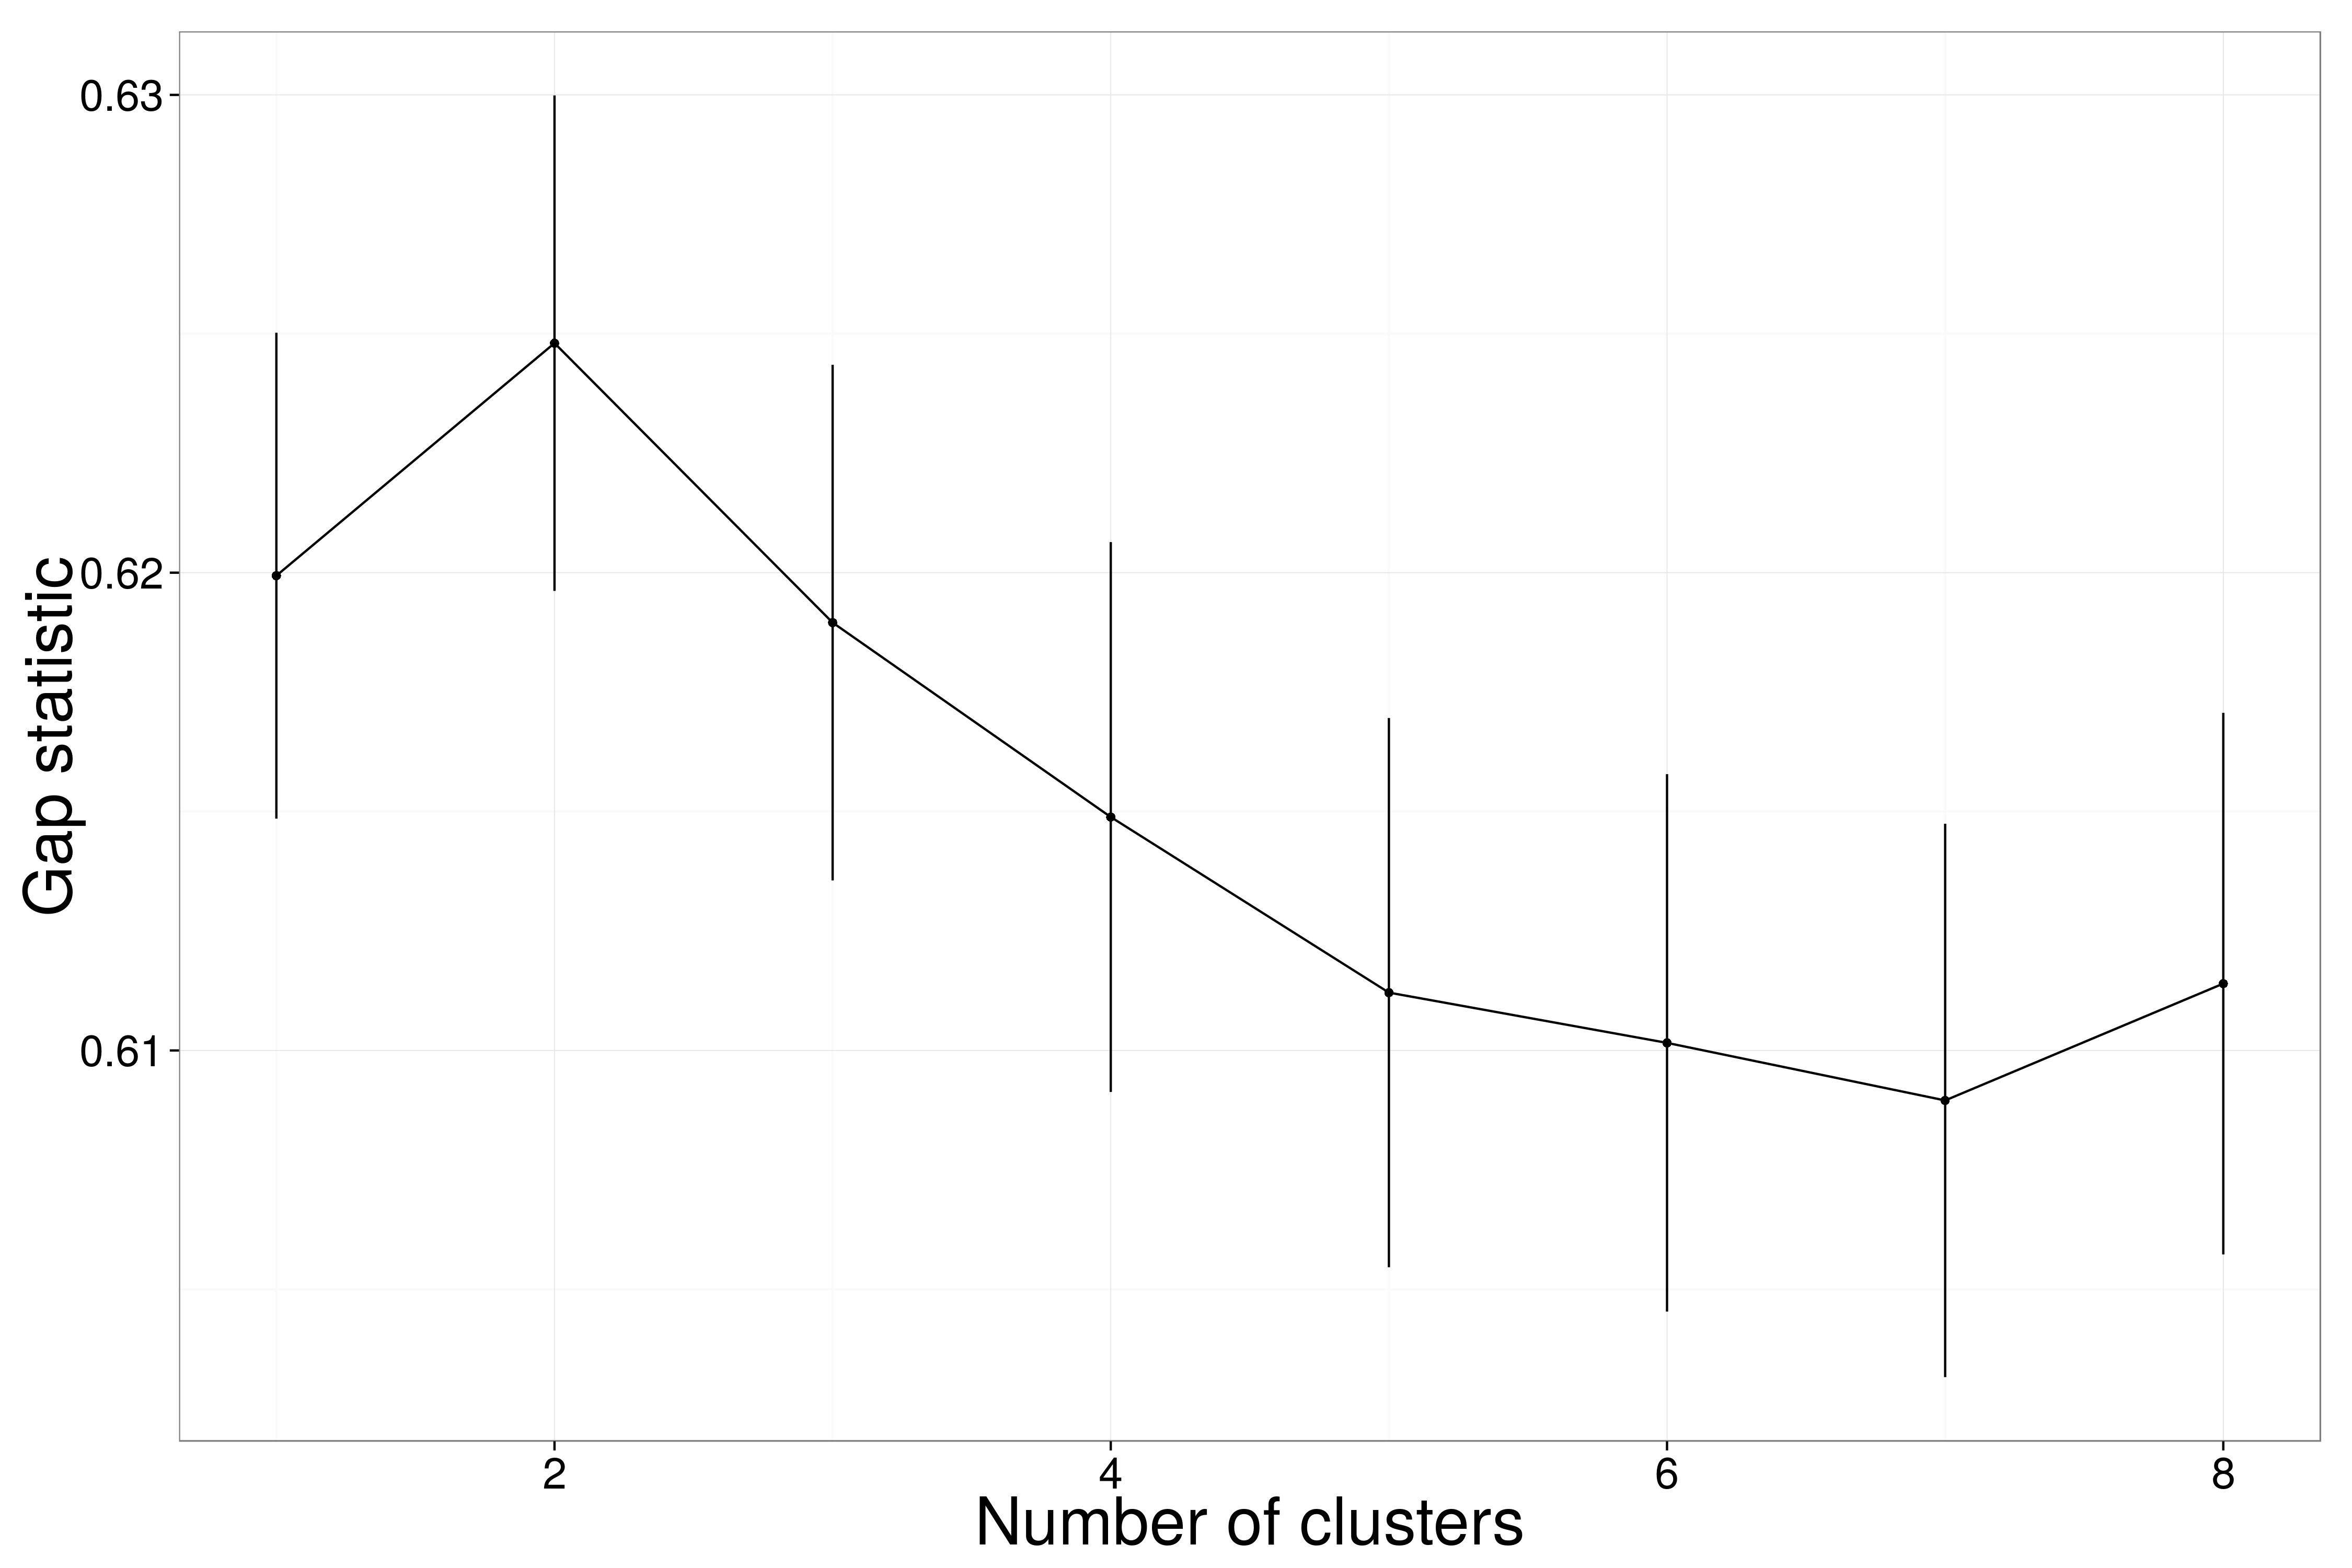
\includegraphics[height = 0.5\textheight, width = \textwidth, keepaspectratio = true]{figure/gap_res}
  \caption{Results from PAM clustering of the Riemannian shape distance for 8 different number of clusters. Vertical lines are 1 standard deviation of the mean determined from 500 resamples.}
  \label{fig:gap}
\end{figure}

Comparison of gap statistic values from PAM clustering show that the optimal, minimal number of clusters is most likely one (Fig. \ref{fig:gap}). There is some ambiguity in choice because, although it is not statistically different from a solution with only one group, the solution with two groupings does have the greatest mean gap statistic. However, there is no geographical signal in the results of this clustering solution (Fig. \ref{fig:gap_map}). Because of this, we assert that there is no means of naturally partitioning plastron shape into distinct subgroups with out reference to external information.

\begin{figure}[ht]
  \centering
  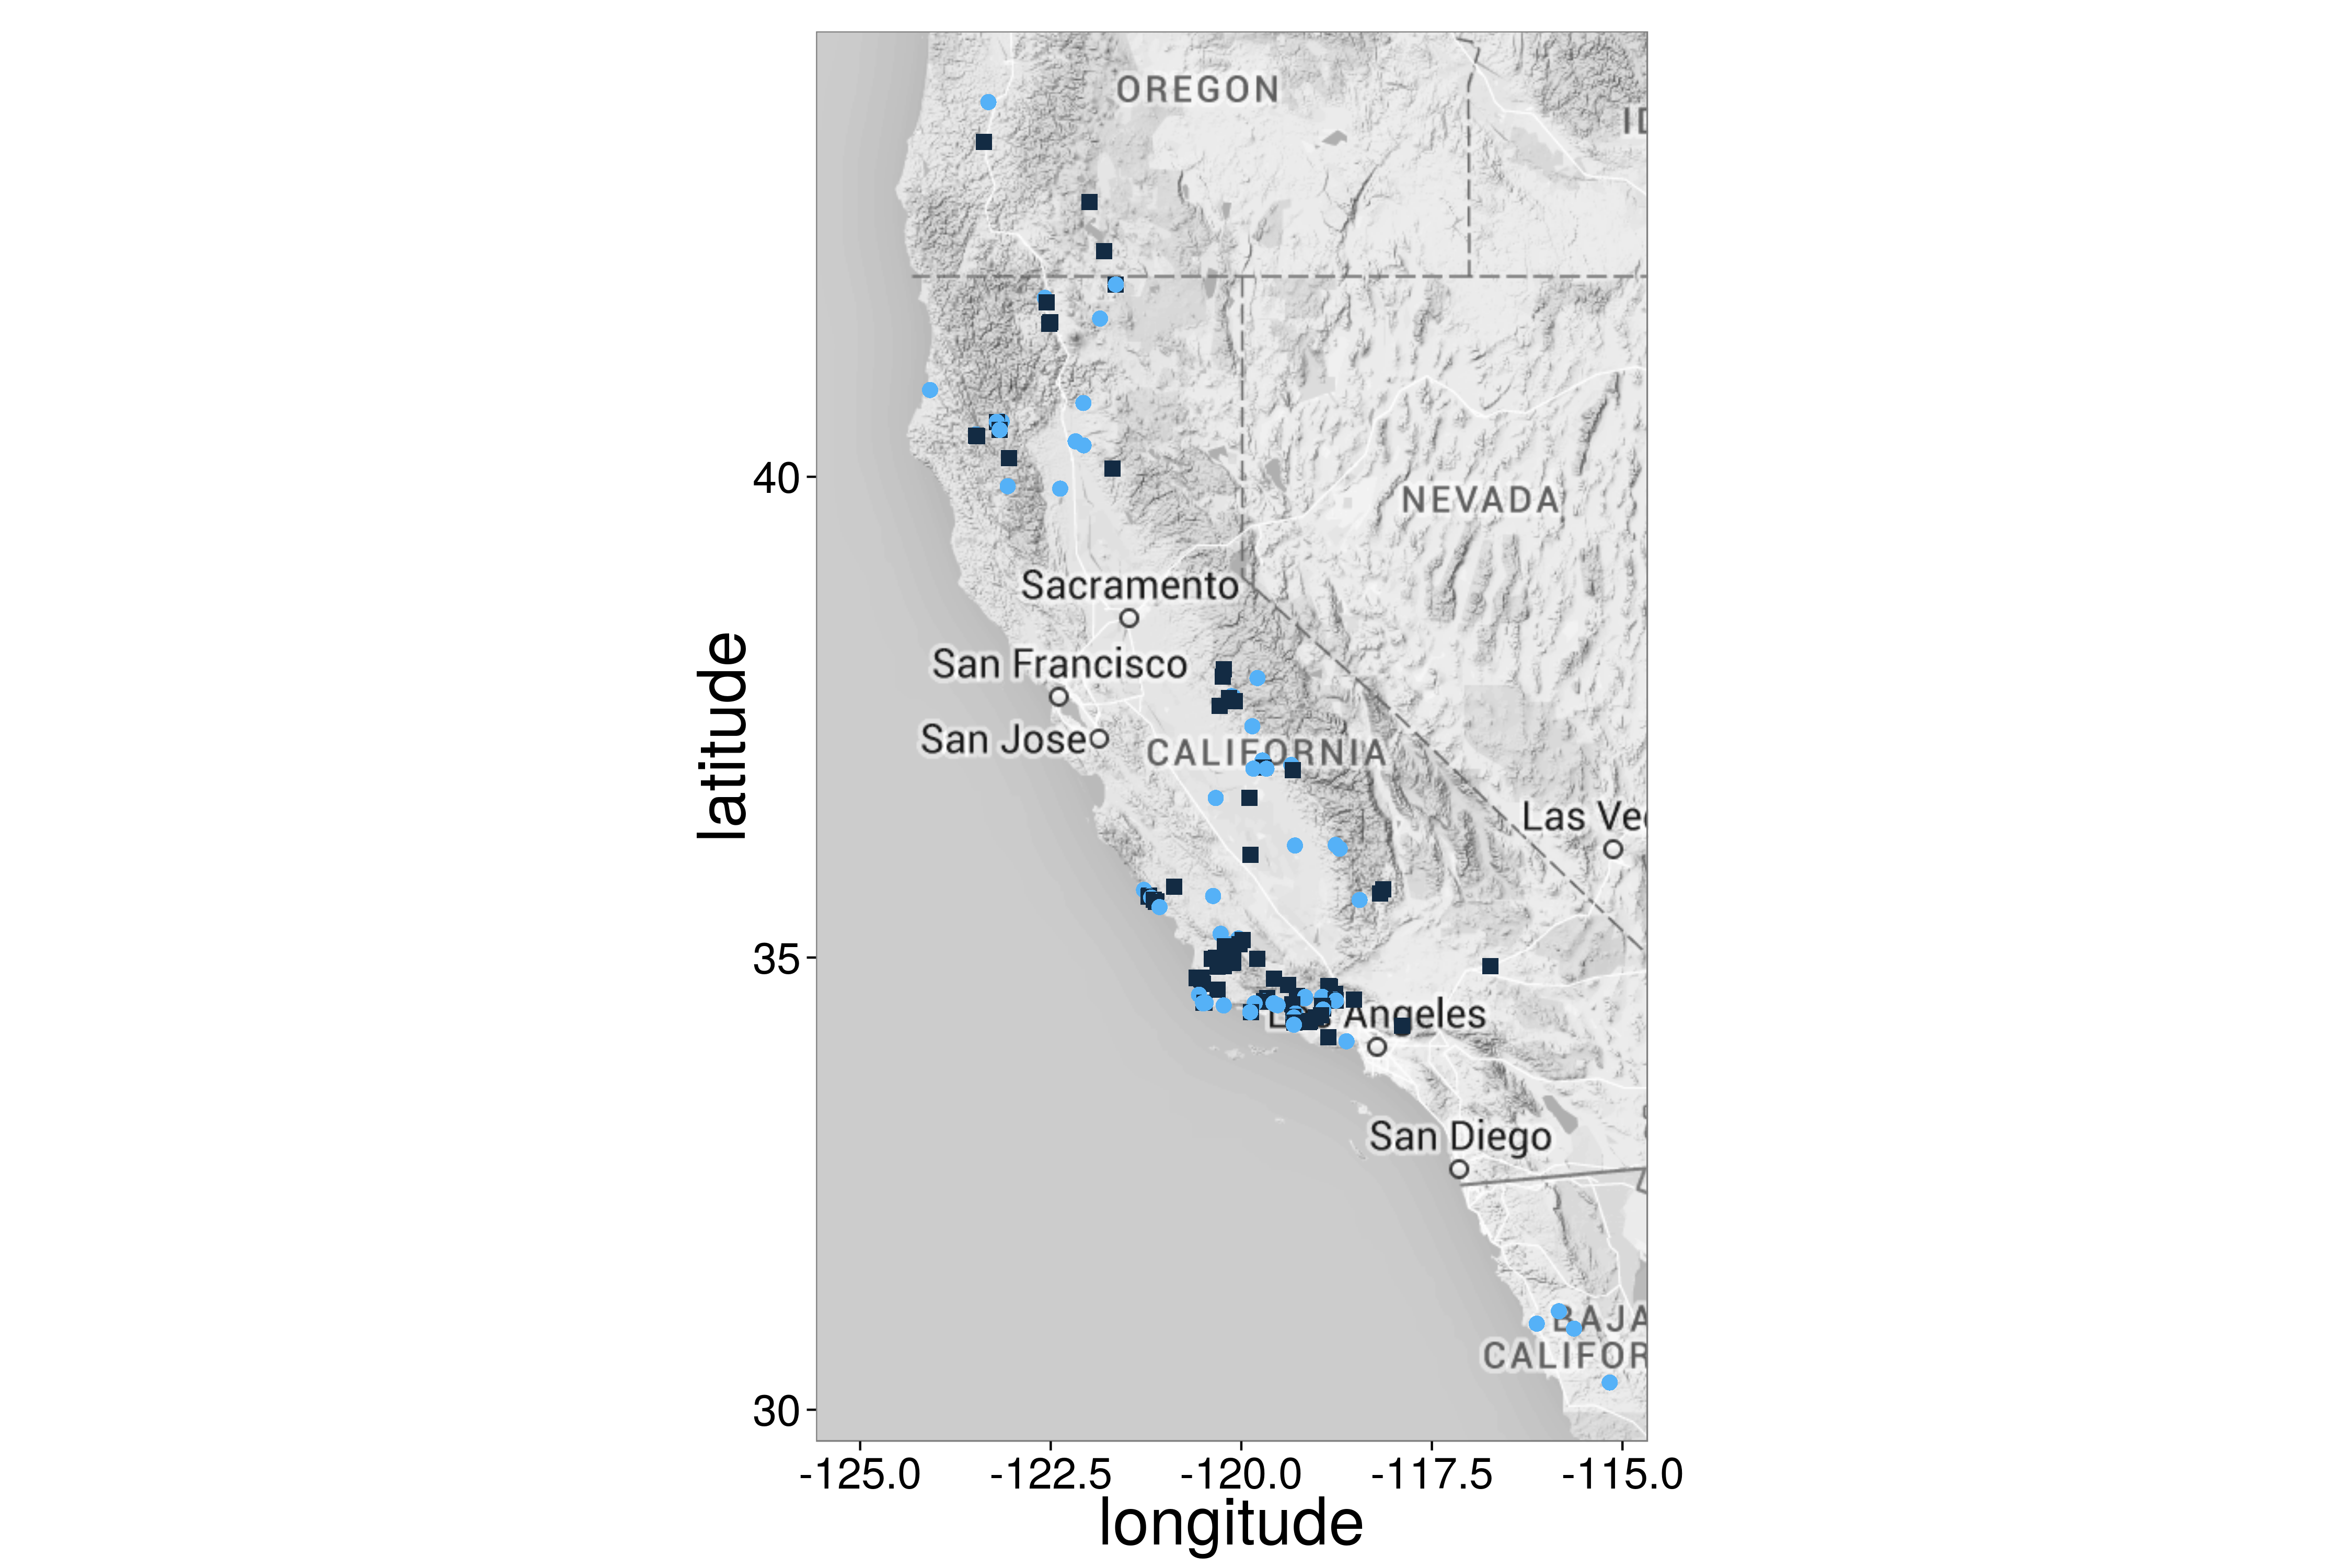
\includegraphics[height = 0.5\textheight, width = \textwidth, keepaspectratio = true]{figure/gap_map}
  \caption{Comparison of geographic distribution of clustered observations from the 2 clustering PAM solution. Colour and shape correspond to each of the groups. There is clearly no geographic signal in the data.}
  \label{fig:gap_map}
\end{figure}


\subsection{Supervised learning}
% model selection/fit
AUC--based model selection revealed some important patterns of variation and congruence between the classification schemes and the actual data. Generally, the best performing models tended to include as many PCs as possible \ref{fig:sel}). Note that the best random forest models were determined via recursive feature selection, so PCs were not included in order of percent variance explained. That almost all LDA and multinomial logistic regression models were as complex as possible indicates that the differences between the different groups within each classification scheme are very small.

\begin{figure}[ht]
  \centering
  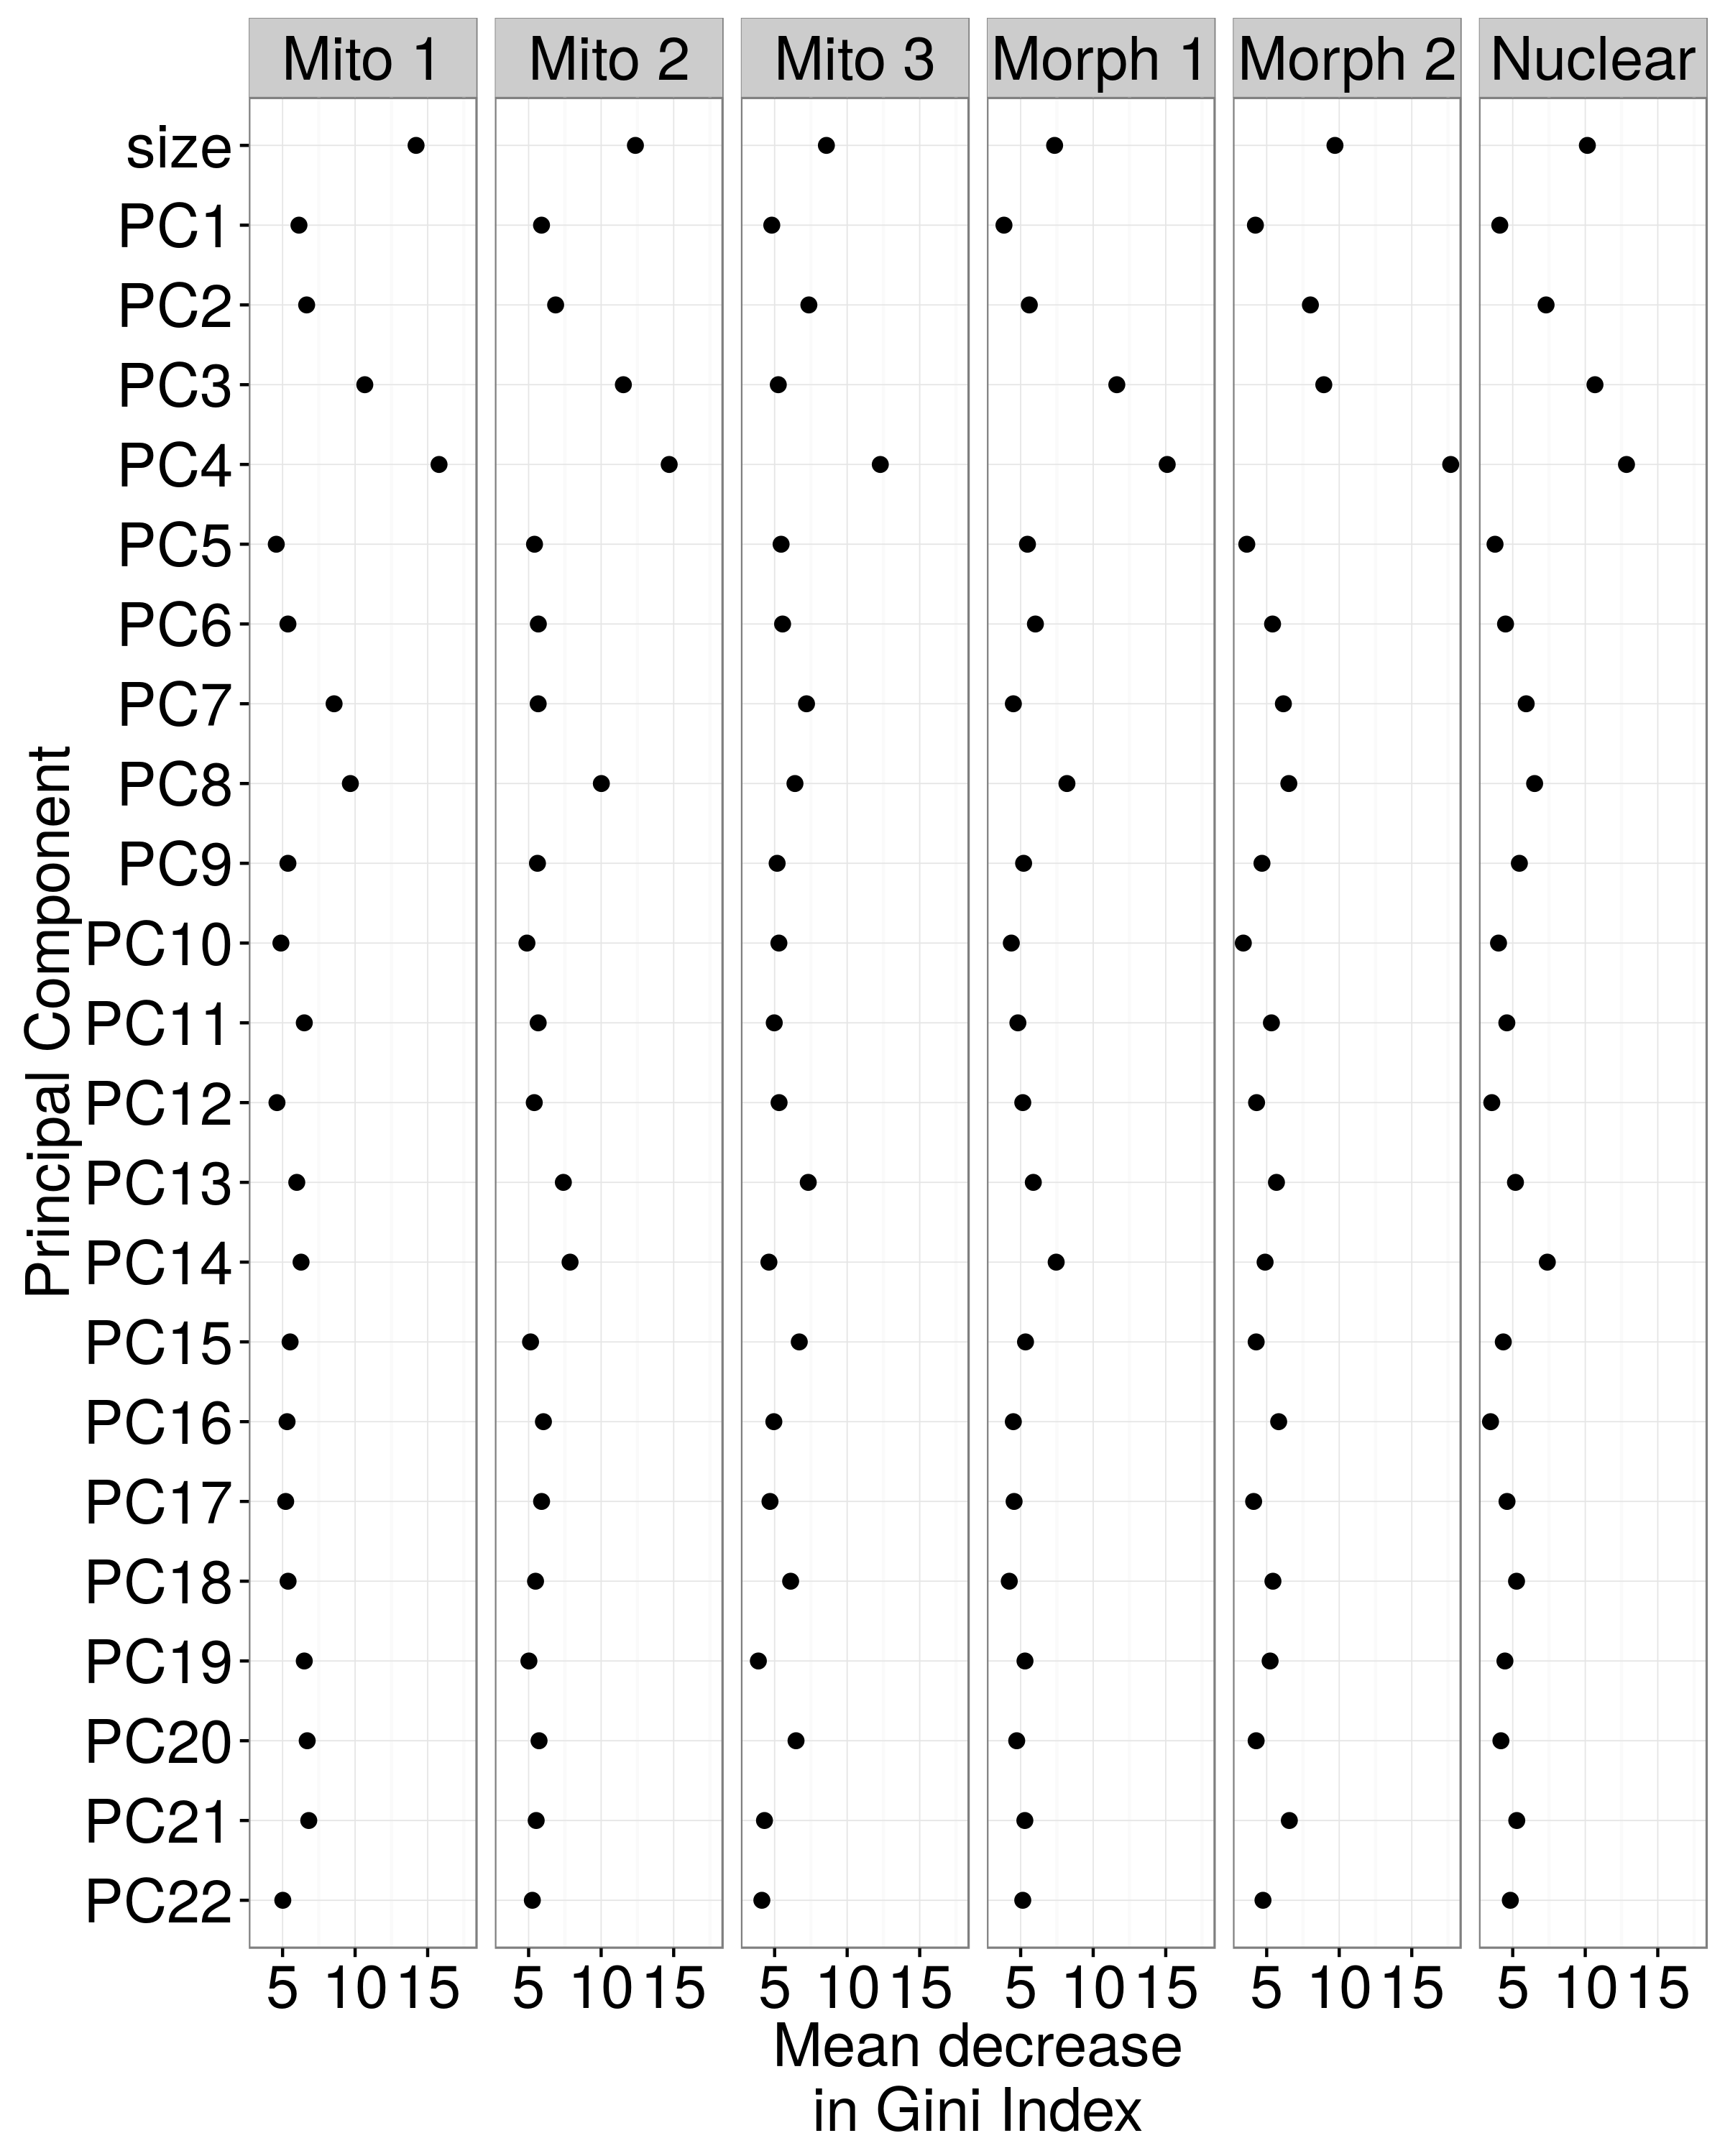
\includegraphics[height = 0.5\textheight, width = \textwidth, keepaspectratio = true]{figure/var_imp}
  \caption{Variable importance from the random forest models for each of the six classification schemes. Importance is measured as the mean decrease in Gini Index, which is a measure of the strength by which that variable determines CART structure. Indices that are farther to the right indicate greater variable importance.}
  \label{fig:var_imp}
\end{figure}

As part of fitting a random forest model, a ranking of variable importance also is determined. Interestingly, the order of variable importance is not the same as the order of the PCs (\ref{fig:var_imp}). This means that the variance describing the differences between the classes does not align with the major axes of variance (i.e. the PCs). Such a result is expected if variation between classes was extremely fine grained and not a part of the principal form or function of the plastron. Moreover, this result is consistent with the results from the AUC--based model selection for the multinomial logistic regression and LDA models.

\begin{figure}[ht]
  \centering
  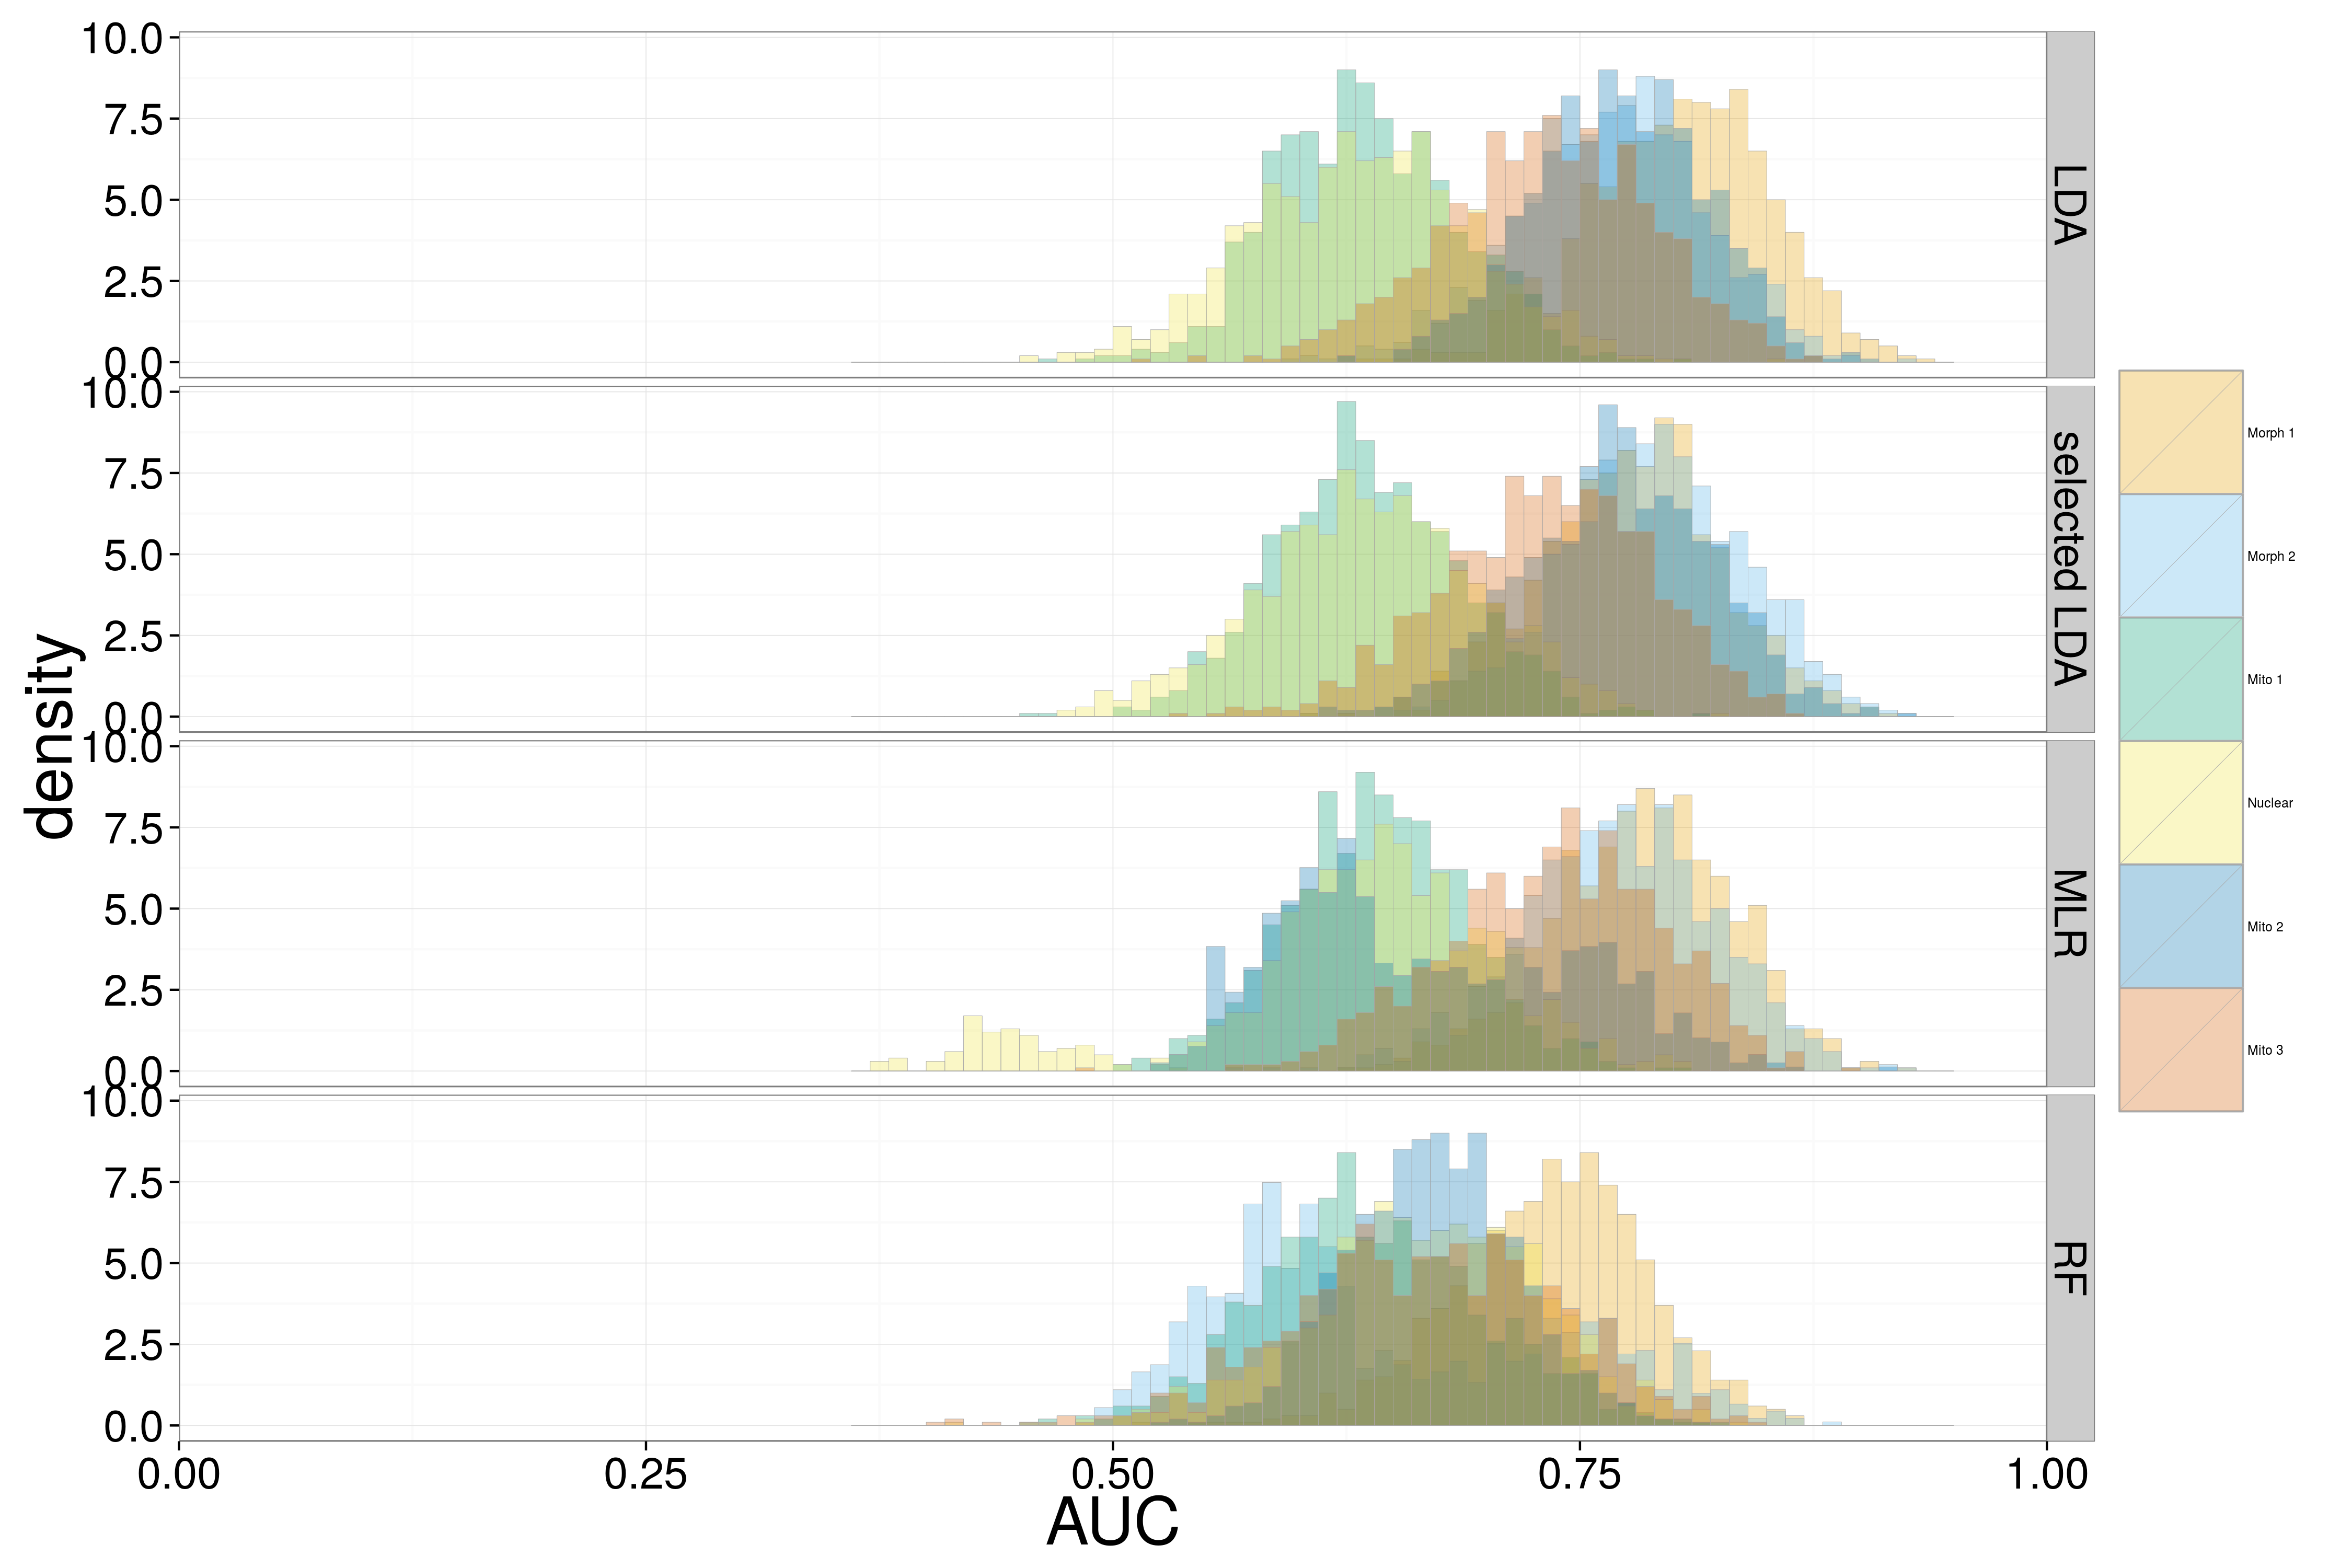
\includegraphics[height = 0.5\textheight, width = \textwidth, keepaspectratio = true]{figure/gen_res}
  \caption{Bootstrap distributions for genearlized AUC values for each of the classification schemes. Each row corresponds to a different modeling approach: multinomial logistic regression (MLR), random forest (RF), linear discriminate analysis (LDA), and LDA using best variables from random forest. Each distribution corresponds to 1000 bootstrap replicates.}
  \label{fig:gen_hist}
\end{figure}

Observed AUC values for all of the optimal models are not exceptionally high (\ref{fig:sel}). In most cases the different proposed classification schemes are generally poor descriptors of the observed variation. It appears that the data set is overwhelmed by noise, making any accurate classifications difficult at best. This observation is cemented with the generalizations of the models to the testing data set (\ref{fig:gen_hist}).

\begin{figure}[ht]
  \centering
  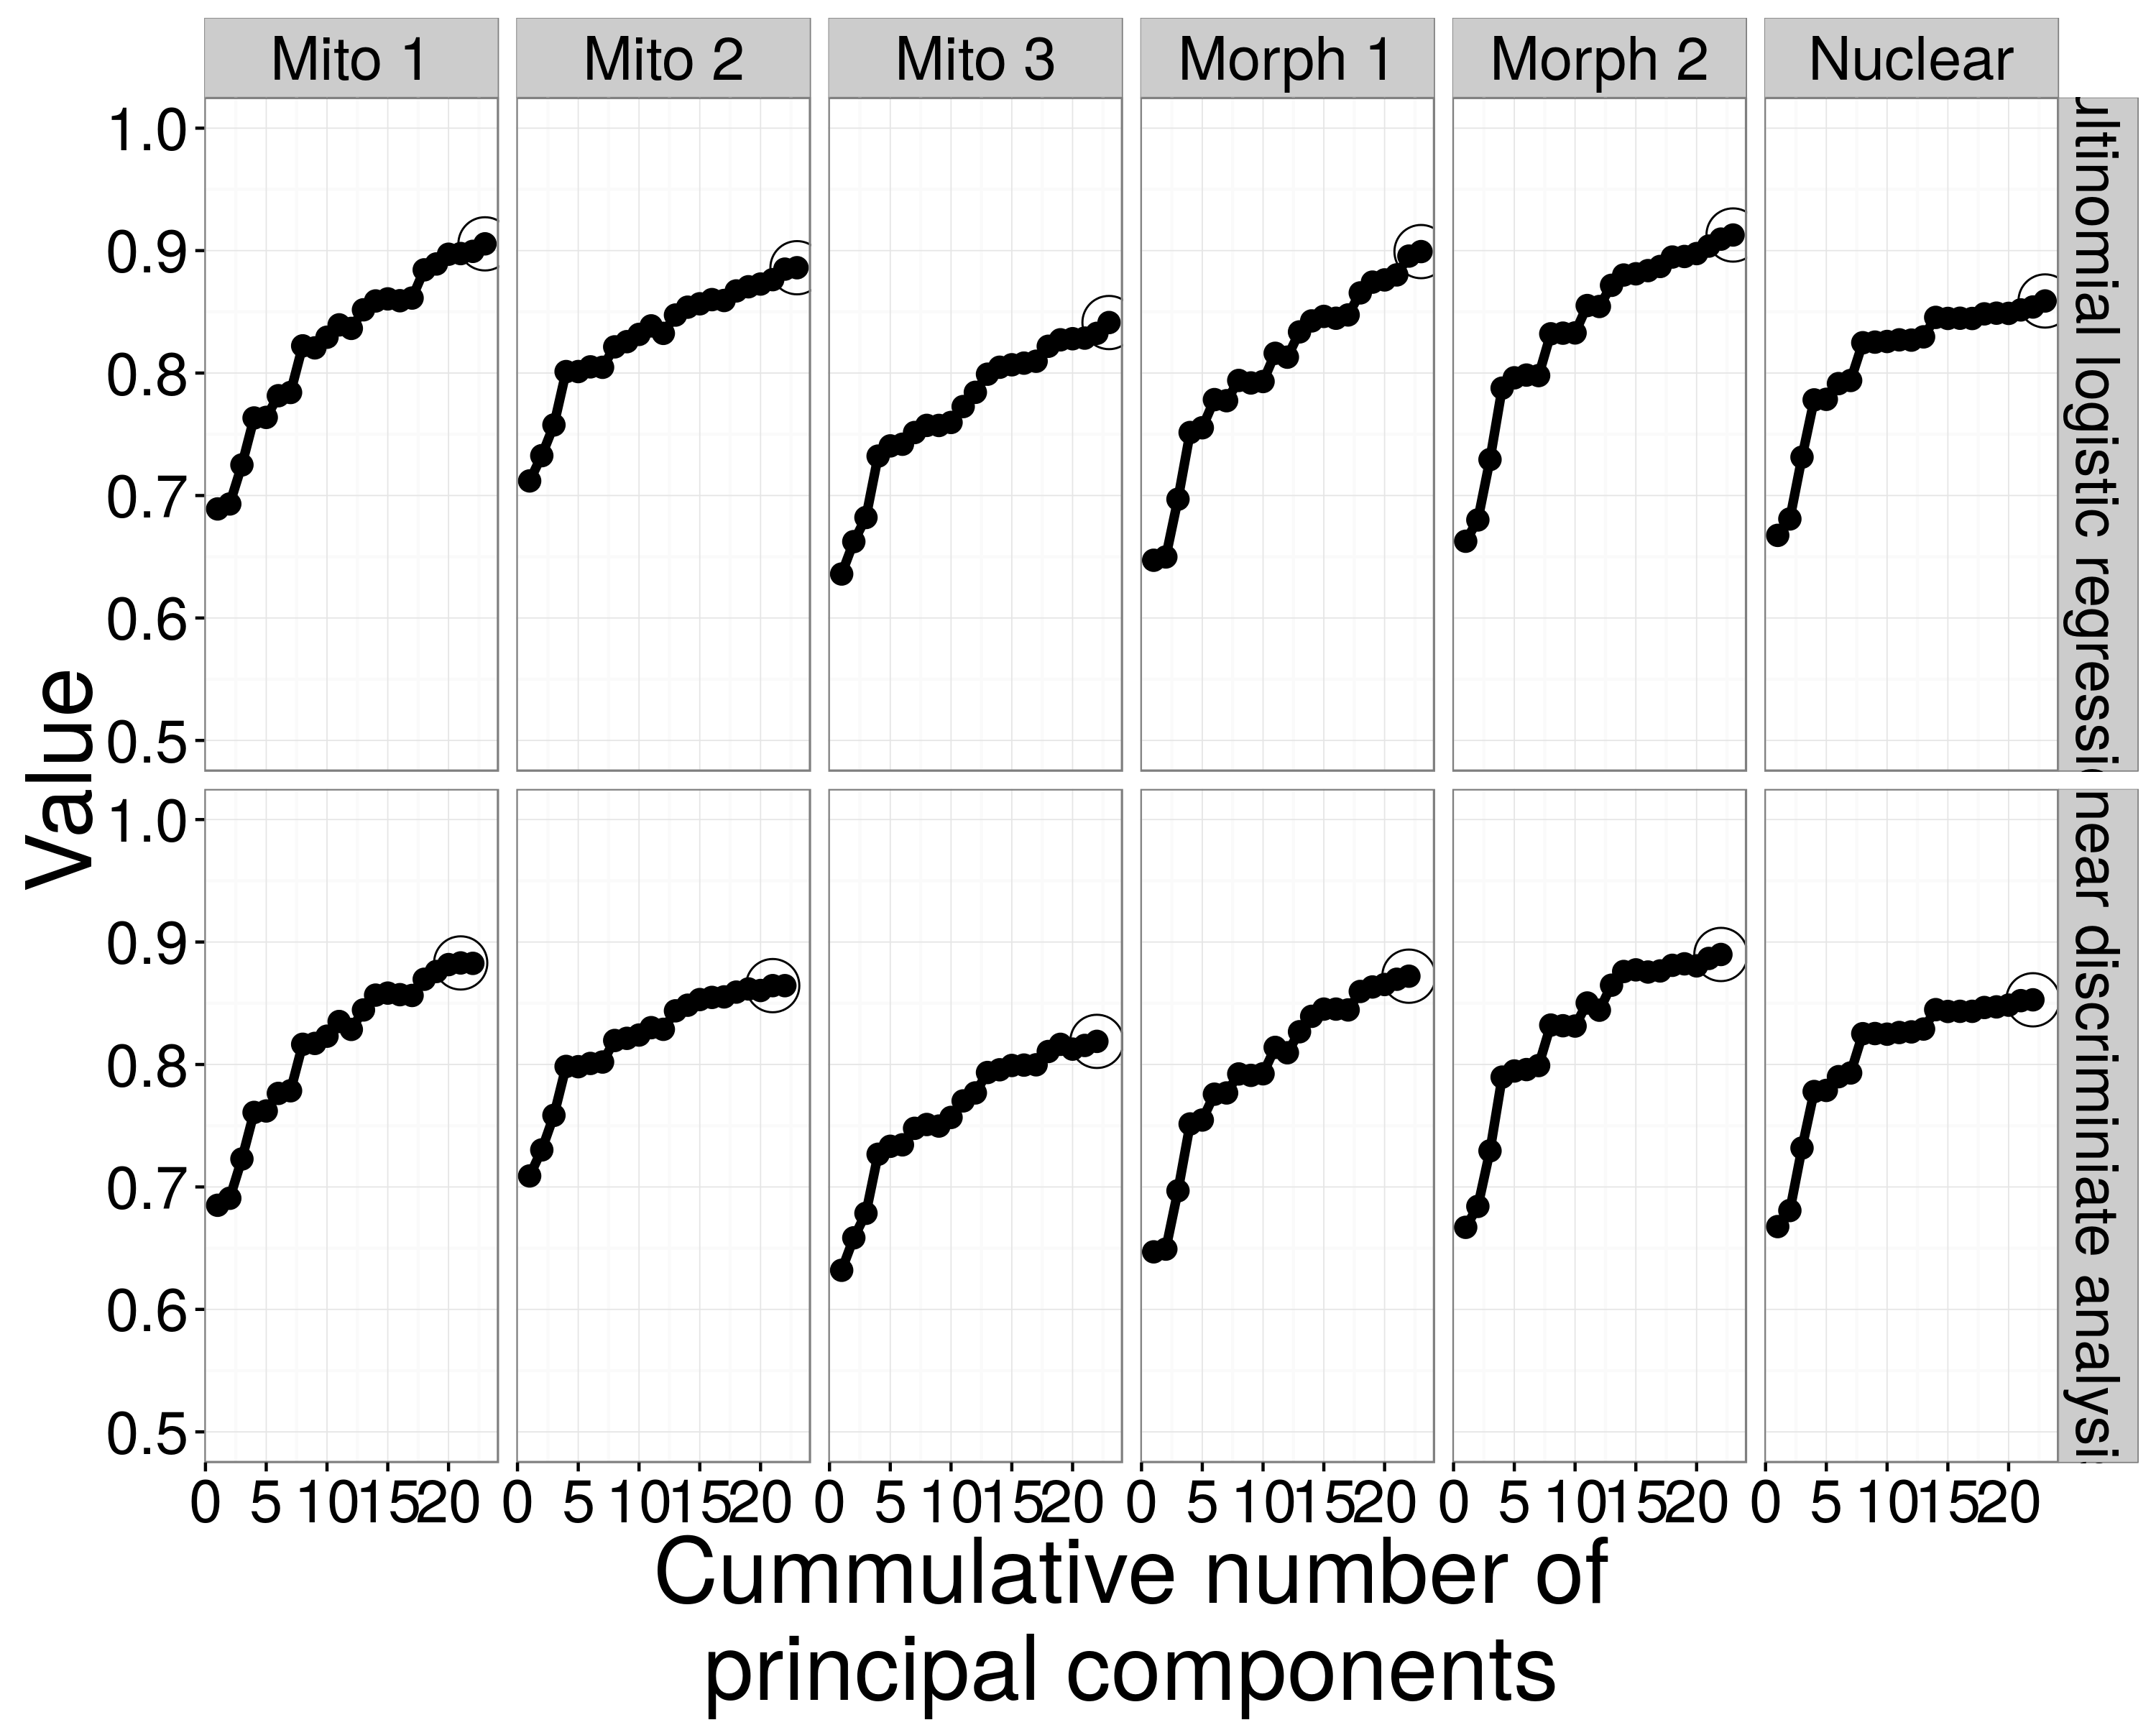
\includegraphics[height = 0.5\textheight, width = \textwidth, keepaspectratio = true]{figure/sel_val}
  \caption{Graphical representation of the AUC values from model selection for multinomial logistic regression and linear discriminate analysis, respecitively. AUC model selection is based on greatest AUC value. The horizontal axis corresponds to the cummulative number of axes included in the model of interest. A highlighted point corresponds to the AUC best model for that classification scheme.}
  \label{fig:sel}
\end{figure}

\begin{table}[ht]
  \centering
  \caption{AUC values for the best model of each classification scheme for both the observed (training) data and the generalized (testing) data. Results from all three different supervised learning approaches are shown here. AUC values range between 0.5 and 1. }
  \begin{tabular}{ l | c c | c c | c c }
    \hline
    & \multicolumn{2}{| l |}{random forest} & 
    \multicolumn{2}{| l |}{multinomial logistic regression} & 
    \multicolumn{2}{| l}{linear discriminate analysis} \\
    Scheme & Observed & Generalized & Observed & Generalized & Observed & Geneeralized \\ 
    \hline
    \hline
    Morph 1 & 0.63 & 0.73 & 0.75 & 0.79 & 0.75 & 0.80 \\ 
    Morph 2 & 0.61 & 0.58 & 0.76 & 0.77 & 0.76 & 0.77 \\ 
    Mito 1& 0.63 & 0.62 & 0.75 & 0.63 & 0.75 & 0.63 \\ 
    Mito 2 & 0.77 & 0.67 & 0.80 & 0.64 & 0.80 & 0.63 \\ 
    Mito 3 & 0.56 & 0.64 & 0.71 & 0.74 & 0.71 & 0.73 \\ 
    Nuclear & 0.56 & 0.67 & 0.74 & 0.62 & 0.74 & 0.77 \\ 
    \hline
  \end{tabular}
  \label{tab:comp}
\end{table}

Mean AUC values for the model generalizations, in most cases, are approximately equal to the observed AUC values from the training data set (Table \ref{tab:comp}). The  cases in which the AUC from the  generalizations is less than the observed, indicate poor model fit and a poor classification scheme. AUC values from model generalization, or estimating testing data set membership, does not indicate a clear ``best'' classification scheme (Fig. \ref{fig:gen_hist}). Although the scheme with two species has the greatest AUC point estimate for each modeling approach, this scheme is not significantly greater than any other except in some limited cases (e.g. LDA, Table \ref{tab:gen_tests}). 

\begin{table}[ht]
  \centering
  \caption{Results of bootstrap comparisons between the scheme with the highest mean AUC value and all other schemes, defined P(best - other \(>\) 0). An asterix indicates the best scheme. This was done for each of the three modeling techniques included in this study: random forest (RF), multinomial logistic regression (MLR), and linear discriminate analysis (LDA). Probabilities are the percent of comparisons that are greater than the observed difference in means.}
  \begin{tabular}{ l r r r }
    \hline
    Scheme & RF & MLR & LDA \\
    \hline
    \hline
    Morph 1 & \(\ast\) & \(\ast\) & 1 \\
    Morph 2 & 0.79 & 0.55 & 1 \\
    Mito 1 & 0.89 & 0.94 & 1 \\ 
    Mito 2 & 0.82 & 0.57 & \(\ast\) \\ 
    Mito 3 & 0.79 & 0.69 & 0.73 \\ 
    Nuclear & 0.79 & 0.96 & 0.96 \\ 
    \hline
  \end{tabular}
  \label{tab:gen_tests}
\end{table}

Differences in mean shape between correctly and incorrectly classified observations from test set frequently were statistically significant, though there are exceptions. Again, this test was to determine if the mean shapes were statistically different or not. The frequency of these results, however, is important because it means that the different models are poor predictors of class membership. This may be because differences in plastron shape do not align with the any of the hypothesized classification schemes.

\subsection{Comparison with clear-cut example}
In contrast with the above results, the analysis of the seven morphologically-distinct species demonstrates near perfect classification of the both the in-sample and out-of-sample datasets (Table \ref{tab:second_res}). Additionally, the distribution of ROC scores from 1000 bootstrap replicates are tightly clustered near ROC = 1 (Fig. \ref{fig:seven_boot}), which is contrast to the results from the \textit{E. marmorata} case (Fig. \ref{fig:gen_hist}). These results demonstrate that when there are strong distinctions between the states of the classification schemes, the methods used here can recover them.

\begin{table}[ht]
  \centering
  \caption{Results from classification model estimates of the secondary, multi-species dataset. Models are random forest (RF), linear discriminate analysis (LDA), and multinomial logistic regression (MLR). Comparison of in-sample and out-of-sample AUC of the best performing model, along with the number of predictors. AUC values range between 0.5 (no better than random) and 1 (perfect classification).}
  \begin{tabular}{ l r r r }
    \hline
    & \# predictors & In-sample AUC & Out-of-sample AUC \\ 
    \hline
    \hline
    RF &   11 & 1.000 & 0.999 \\ 
    MLR &    6 & 1.000 & 0.998 \\ 
    LDA &   10 & 1.000 & 1.000 \\ 
    \hline
  \end{tabular}
  \label{tab:second_res}
\end{table}

\begin{figure}[ht]
  \centering
  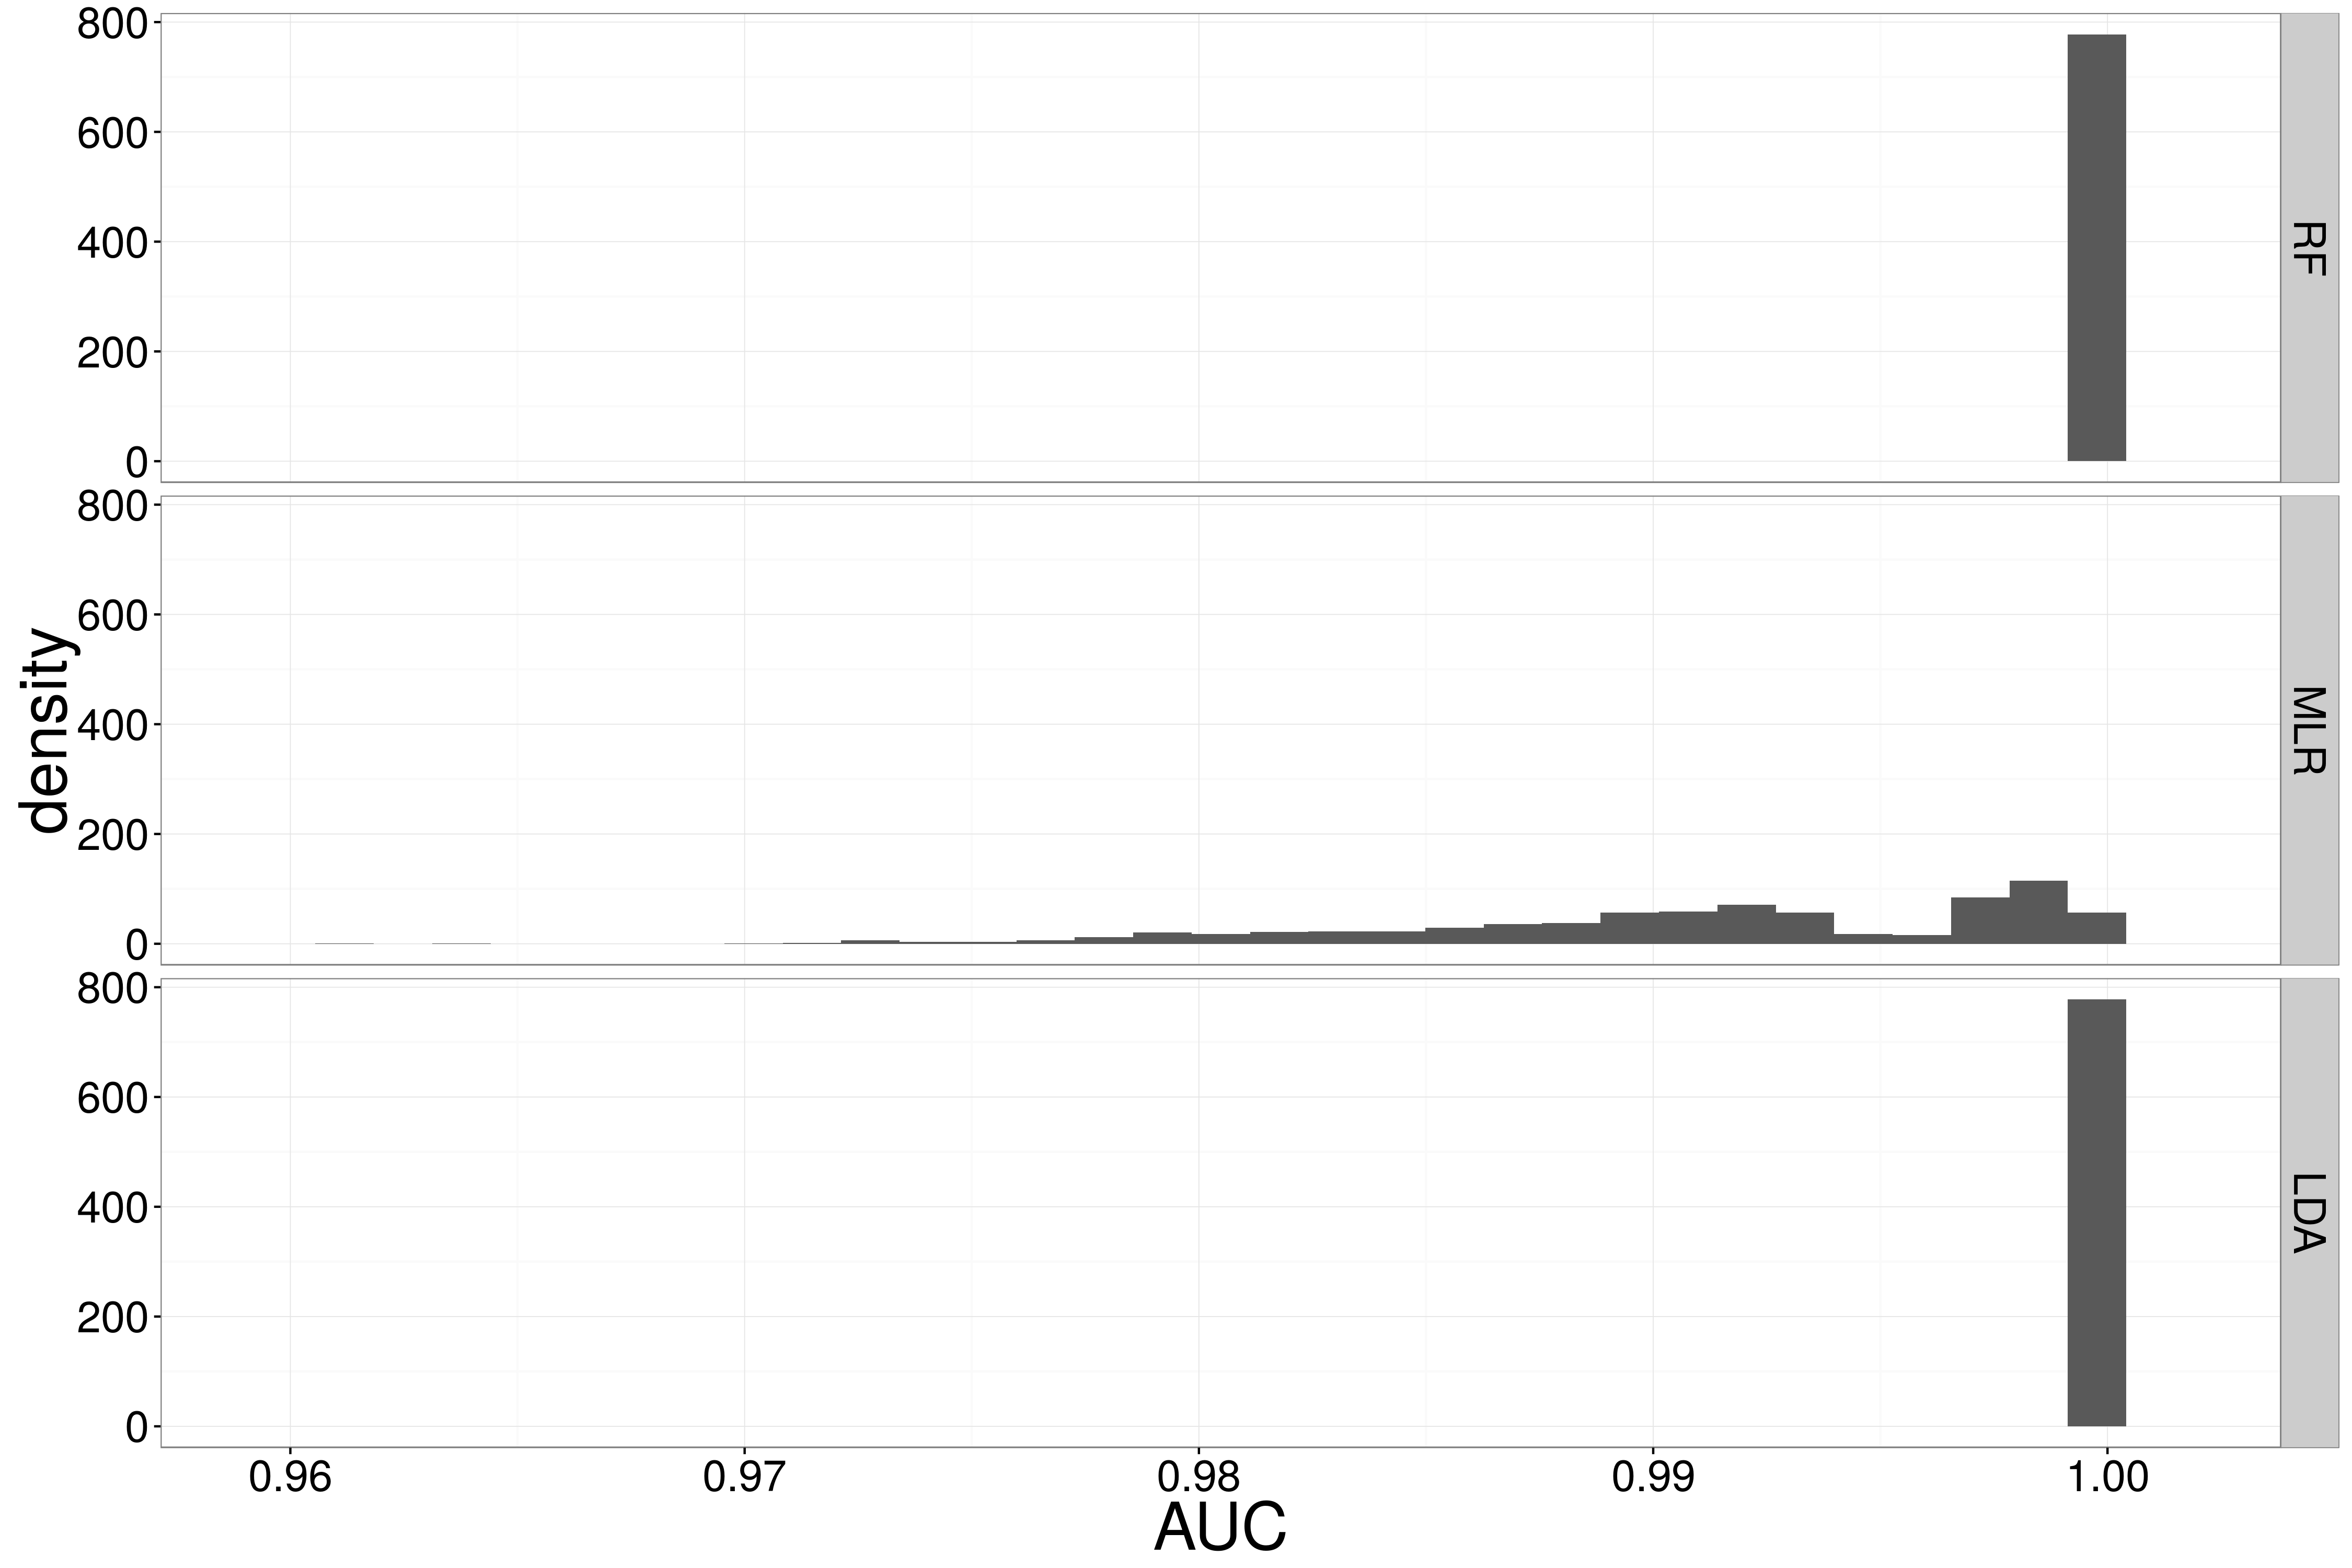
\includegraphics[height = 0.5\textheight, width = \textwidth, keepaspectratio = true]{figure/seven_boot}
  \caption{Distribution of 1000 bootstrap replicates of the out-of-sample AUC values from the secondary, multi-species dataset. The AUC values are from the random forest (RF), linear discriminate analysis (LDA), and multinomial logistic regression (MLR). AUC values range between 0.5 (no better than random) and 1 (perfect classification).}
  \label{fig:seven_boot}
\end{figure}


\section{Discussion}

The results of this study indicate that there is no clear grouping of \textit{E. marmorata} based on plastron shape.

The unsupervised learning results indicate only a single group of observations being optimal, which is consistent with the results from the generalizations of the supervised learning models. The classification schemes used in the supervised learning models correspond, loosely, to unsupervised learning solutions with multiple groups. Because unsupervised learning solutions with multiple groups are poor descriptors of the observed variation, it is important to see this generally supported by the supervised learning results.

The results from fitting the various supervised learning models to each of the classification schemes generally shows that no one scheme is ``best.'' Possible explanations include that the genetic differentiation is not associated with plastron shape variation and/or that local selective pressures (e.g. from hydrological regime) overwhelm morphological differentiation. This makes sense given that the plastron is involved in both protection and hydrodynamics, and not necessary mate choice \citep{Rivera2008,Rivera2011,Stayton2011,Rivera2014} and that shell shape in \textit{E. marmorata} is known to vary among populations inhabiting water bodies with different flow regimes \citep{Holland1992,Lubcke2007,Germano2009}. Plastron shape does not seem to preserve a strong phylogenetic signal at the interspecific level in emydine turtles \citep{Angielczyk2011}, and our current results suggest that this may be the case for phylogeographic signal within emydine species as well. A final possibility (explored below) is that the proposed classification schemes themselves do not represent significant evolutionary lineages.

Both the low AUC values (\(< 0.9\)) and the significant difference between the correctly and incorrectly classified observations support the conclusion that none of the hypothesized classification schemes are good descriptors of the observed plastral variation within \textit{E. marmorata}.

Nevertheless, it is important to note that plastron shape is an extremely effective method for differentiating members of the other seven species we investigated. The magnitude of shape differences between the species (measured as Procrustes distance between species' mean shapes) is approximately an order of magnitude greater than the differences between the \textit{E. marmorata} subgroups, and the machine learning methods had no trouble accurately classifying the specimens correctly. These results demonstrate that plastron shape is normally a good marker for species delineation iin the closest relatives of \textit{E. marmorata}, and that our lack of results for \textit{E. marmorata} is not simply a shortcoming of the methods we applied. Indeed, they beg the question of what factors have suppressed morphological differentiation of plastron shape in \textit{E. marmorata} and \textit{E. pallida} if they are distinct species. Invoking issues such as the role of the plastron in protection or the need for streamlining are insufficient because the other species are expected to be subject to similar constraints \citep{Stayton2011,Pollyb}. 

\subsection{Is there more than one species of Western Pond Turtle?}

The lack of morphological support for the distinctiveness of \textit{E. pallida} does not, on its own, preclude the recognition of this taxon. However, this apparent lack of congruence does prompt a reexamination of the methods and concepts that led to that taxonomic revision, especially considering that plastron shape is normally a strong indicator of species differences amoung emydines. In other words, before we can assess the significance of the morphological non-diagnosablity, it is essential to evaluate the methods and concepts that led to the initial taxonomic revision. 

\citet{Spinks2014} elevated \textit{E. pallida} based on a Bayesian species delimitation analysis of SNP data using BPP \citep{Yang2010b}. However, \citet{Spinks2014} did not heed the caveats about species delimitation methods raised by \citet{Carstens2013}. In addition to specifically addressing the shortcomings of validation methods such as BPP that rely on guide trees and ``should be interpreted with caution,'' \citet{Carstens2013} also strongly emphasize that ``Inferences regarding species boundaries based on genetic data alone are likely inadequate, and species delimitation should be conducted with consideration of the life history, geographical distribution, morphology and behaviour (where applicable) of the focal system\dots'' These caveats evoke the development of the Unified Species Concept \citep{Dayrat2005a,DeQueiroz2007b}, Integrative Taxonomy \citep{Padial2010}, and other pluralist approaches to species delimitation. None of these considerations were brought to bear on the \textit{E. marmorata} system until now, and in doing so we find the proposal that \textit{E. pallida} is a distinct species to be lacking in a normally robust morphological marker.

The natural history and geographical distribution of \textit{E. marmorata} and \textit{E. pallida} also make the recognition of these taxa implausible. The data from \citet{Spinks2014} show extensive introgression and admixture in Central California, which is expected because there are no significant barriers to gene flow in this region. Combined with the well-demonstrated ability for testudinoid turtles, including emydids and even \textit{Emys}, to hybridize (e.g. \citealt{Buskirk2005,Spinks2009,Parham2013}) it is hard to imagine how \textit{E. marmorata} and \textit{E. pallida} could maintain their integrity in the face of such admixture. Because the geography, natural history, demonstrated genetic admixture of \textit{E. marmorata}, and comparisons with other morphologically-diagnosable species conflict with the recognition of \textit{E. pallida}, we hypothesize that out inability to classify the morphological data by proposed species is because \textit{E. pallida} is not a distinct species. We agree with \citet{Carstens2013} that ``the inferences drawn from species delimitation studies should be conservative, for in most contexts it is better to fail to delimit species than it is to falsely delimit entities that do not represent actual evolutionary lineages.'' 

We fully agree with \citet{Spinks2014} that \textit{E. marmorata} (\textit{sensu lato}) is a species deserving of strong conservation efforts, and we do not wish to trivialize this need. Moreover, the genetic diversity uncovered by the analysis of \citet{Spinks2014} should be explicitly accounted for in any conservation plan. Given the apparent lack of morphological distinction, however, we consider that this diversity should be considered Evolutionary Significant Units or Distinct Population Segments instead of distinct species.

Finally, it is important to note that the data and analyses we present do not let us definitively say whether the apparent lack of morphological divergence within \textit{E. marmorata} truly reflects the presence of a single species, or if it is an artifact of plastron shape being a poor morphological marker for phylogenetic and phylogeographic divergences, because we could not carry out our morphometric analyses on the specimens from which the genetic data were obtained. The comparisons with the other emydine species, suggests it is because \textit{E. marmorata} is a single species. However, tests of both our preferred conclusion (\textit{E. marmorata} as a single species) and that \citet{Spinks2014} should include morphological and molecular analyses of the same set of voucher specimens, as well as additional tests of species delimitation using alternative methods and corroborating evidence as suggested by \citet{Carstens2013}. From a morphological standpoint, support for the validity of ``\textit{E. Pallida}'' may come from other aspects of morphology, such as carapace shape or other features. Likewise, further investigation of the phylogeographic utility of plastron shape in other turtle species will help to clarify whether the lack of differentiation seen in \textit{E. marmoarata}, and the strong differentiation among the other emydines, is typical or an unusual case.


\section*{Acknowledgements}
Data collection for this project was supported in part by NSF DBI-0306158 (to KDA). G. Miller assisted with data collection and her participation in this research was supported by NSF REU DBI-0353797 (to R. Mooi of CAS). For access to emydine specimens, we thank: J. Vindum and R. Drewes (CAS); A. Resetar (FMNH); R. Feeney (LACM); C. Austin (LSUMNS); S. Sweet (MSE); J.McGuire and C. Conroy (MVZ); A. Wynn (NMNH); P. Collins (SBMNH); B. Hollingsworth (SDMNH); P. Holroyd (UCMP). We are grateful for S. Sweet for field assistance and the California Department of Fish and Game for permits.

\clearpage
\begin{thebibliography}{77}
\providecommand{\natexlab}[1]{#1}
\providecommand{\selectlanguage}[1]{\relax}
\providecommand{\bibAnnoteFile}[1]{%
  \IfFileExists{#1}{\begin{quotation}\noindent\textsc{Key:} #1\\
  \textsc{Annotation:}\ \input{#1}\end{quotation}}{}}
\providecommand{\bibAnnote}[2]{%
  \begin{quotation}\noindent\textsc{Key:} #1\\
  \textsc{Annotation:}\ #2\end{quotation}}

\bibitem[{Angielczyk and Feldman(2013)}]{Angielczyk2013a}
Angielczyk, K.~D. and C.~R. Feldman. 2013. {Are diminutive turtles
  miniaturized? The ontogeny of plastron shape in emydine turtles}. Biological
  Journal of the Linnean Society 108:727--755.
\bibAnnoteFile{Angielczyk2013a}

\bibitem[{Angielczyk et~al.(2011)Angielczyk, Feldman, and
  Miller}]{Angielczyk2011}
Angielczyk, K.~D., C.~R. Feldman, and G.~R. Miller. 2011. {Adaptive evolution
  of plastron shape in emydine turtles.} Evolution 65:377--394.
\bibAnnoteFile{Angielczyk2011}

\bibitem[{Angielczyk and Sheets(2007)}]{Angielczyk2007}
Angielczyk, K.~D. and H.~D. Sheets. 2007. {Investigation of simulated tectonic
  deformation in fossils using geometric morphometrics}. Paleobiology
  33:125--148.
\bibAnnoteFile{Angielczyk2007}

\bibitem[{Baird and Girard(1852)}]{Baird1852}
Baird, S.~F. and C.~Girard. 1852. {Descriptions of new species of reptiles
  collected by the U.S. Exploring Expedition under the command of Capt. Charles
  Wilkes}. Proceedings of the National Academy of Sciences Philadelphia
  6:174--177.
\bibAnnoteFile{Baird1852}

\bibitem[{Bauer et~al.(2000)Bauer, Parham, Brown, Stuart, Grismer, Papenfuss,
  Bohme, Savage, Carranza, Grismer, Wagner, Schmitz, Ananjeva, and
  Inger}]{Bauer2000}
Bauer, A.~M., J.~F. Parham, R.~M. Brown, B.~L. Stuart, L.~Grismer, T.~J.
  Papenfuss, W.~Bohme, J.~M. Savage, S.~Carranza, J.~L. Grismer, P.~Wagner,
  A.~Schmitz, N.~B. Ananjeva, and R.~F. Inger. 2000. {Availability of new
  Baysian-delimited gecko names and the importance of character-based species
  descriptions}. Proceedings of the Royal Society B: Biological Sciences
  278:490--492.
\bibAnnoteFile{Bauer2000}

\bibitem[{Baylac et~al.(2003)Baylac, Villemant, and Simbolotti}]{Baylac2003}
Baylac, M., C.~Villemant, and G.~Simbolotti. 2003. {Combining geometric
  morphometrics with pattern recognition for the investigation of species
  complexes}. Biological Journal of the Linnean Society 80:89--98.
\bibAnnoteFile{Baylac2003}

\bibitem[{Bickford et~al.(2007)Bickford, Lohman, Sodhi, Ng, Meier, Winker,
  Ingram, and Das}]{Bickford2007}
Bickford, D., D.~J. Lohman, N.~S. Sodhi, P.~K.~L. Ng, R.~Meier, K.~Winker,
  K.~K. Ingram, and I.~Das. 2007. {Cryptic species as a window on diversity and
  conservation.} Trends in ecology \& evolution 22:148--55.
\bibAnnoteFile{Bickford2007}

\bibitem[{Breiman(2001)}]{Breiman2001}
Breiman, L. 2001. {Random Forests}. Machine Learning 45:5--32.
\bibAnnoteFile{Breiman2001}

\bibitem[{Breiman et~al.(1984)Breiman, Friedman, Stone, and
  Olshen}]{Breiman1984}
Breiman, L., J.~Friedman, C.~J. Stone, and R.~A. Olshen. 1984. {Classification
  and regression trees}. Wadsworth International Group, Belmont.
\bibAnnoteFile{Breiman1984}

\bibitem[{Bury et~al.(2010)Bury, Germano, and Bury}]{Bury2010}
Bury, R.~B., D.~J. Germano, and G.~W. Bury. 2010. {Population Structure and
  Growth of the Turtle Actinemys marmorata from the Klamath–Siskiyou
  Ecoregion: Age, Not Size, Matters}. Copeia 2010:443--451.
\bibAnnoteFile{Bury2010}

\bibitem[{Buskirk et~al.(2005)Buskirk, Parham, and Feldman}]{Buskirk2005}
Buskirk, S.~W., J.~F. Parham, and C.~R. Feldman. 2005. {On the hybridisation
  between two distantly related Asian turtles (Testudines: Scalia x Mauremys)}.
  Salamandra 41:21--26.
\bibAnnoteFile{Buskirk2005}

\bibitem[{Cardini et~al.(2009)Cardini, Nagorsen, O'Higgins, Polly, {Thorington
  Jr}, and Tongiorgi}]{Cardini2009a}
Cardini, A., D.~Nagorsen, P.~O'Higgins, P.~D. Polly, R.~W. {Thorington Jr}, and
  P.~Tongiorgi. 2009. {Detecting biological distinctiveness using geometric
  morphometrics: an example case from the Vancouver Island marmot}. Ethology
  Ecology \& Evolution 21:209--223.
\bibAnnoteFile{Cardini2009a}

\bibitem[{Carstens and Dewey(2010)}]{Carstens2010}
Carstens, B.~C. and T.~A. Dewey. 2010. {Species Delimitation Using a Combined
  Coalescent and Information-Theoretic Approach: An Example from North American
  Myotis Bats}. Systematic Biology 59:400--414.
\bibAnnoteFile{Carstens2010}

\bibitem[{Carstens et~al.(2013)Carstens, Pelletier, Reid, and
  Satler}]{Carstens2013}
Carstens, B.~C., T.~a. Pelletier, N.~M. Reid, and J.~D. Satler. 2013. {How to
  fail at species delimitation.} Molecular ecology 22:4369--83.
\bibAnnoteFile{Carstens2013}

\bibitem[{Caumul and Polly(2005)}]{Caumul2005a}
Caumul, R. and P.~D. Polly. 2005. {Phylogenetic and environmental components of
  morphological variation: skull, mandible, and molar shape in marmots
  (Marmota, Rodentia).} Evolution; international journal of organic evolution
  59:2460--72.
\bibAnnoteFile{Caumul2005a}

\bibitem[{Clare(2011)}]{Clare2011}
Clare, E.~L. 2011. {Cryptic species? Patterns of maternal and paternal gene
  flow in eight neotropical bats.} PloS one 6:e21460.
\bibAnnoteFile{Clare2011}

\bibitem[{Dayrat(2005)}]{Dayrat2005a}
Dayrat, B. 2005. {Towards integrative taxonomy}. Biological Journal of the
  Linnean Society 85:407--415.
\bibAnnoteFile{Dayrat2005a}

\bibitem[{{De Queiroz}(2007)}]{DeQueiroz2007b}
{De Queiroz}, K. 2007. {Species concepts and species delimitation.} Systematic
  Biology 56:879--86.
\bibAnnoteFile{DeQueiroz2007b}

\bibitem[{Demandt and Bergek(2009)}]{Demandt2009}
Demandt, M.~H. and S.~Bergek. 2009. {Identification of cyprinid hybrids by
  using geometric morphometrics and microsatellites}. Journal of Applied
  Ichthyology 25:695--701.
\bibAnnoteFile{Demandt2009}

\bibitem[{Dobigny et~al.(2003)Dobigny, Granjon, Aniskin, Ba, and
  Voloboulev}]{Dobigny2003}
Dobigny, G., L.~Granjon, V.~Aniskin, K.~Ba, and V.~Voloboulev. 2003. {A new
  sigling species of Taterillus (Muridae, Gerbillinae) from West Agrica}.
  Mammalian Biology 68:299--316.
\bibAnnoteFile{Dobigny2003}

\bibitem[{Dryden(2013)}]{Dryden2013}
Dryden, I.~L. 2013. shapes: Statistical shape analysis. R package version
  1.1-8.
\bibAnnoteFile{Dryden2013}

\bibitem[{Dryden and Mardia(1998)}]{Dryden1998a}
Dryden, I.~L. and K.~Y. Mardia. 1998. {Statistical shape analysis}. Wiley, New
  York.
\bibAnnoteFile{Dryden1998a}

\bibitem[{Eldredge and Gould(1972)}]{Eldredge1972}
Eldredge, N. and S.~J. Gould. 1972. {Punctuated equilibria: an alternative to
  phyletic gradualism}. Pages~82--115 \emph{in} Models in Paleobiology
  (T.~J.~M. Schopf, ed.). Freeman Cooper, San Francisco.
\bibAnnoteFile{Eldredge1972}

\bibitem[{Feldman and Parham(2002)}]{Feldman2002}
Feldman, C.~R. and J.~F. Parham. 2002. {Molecular phylogenetics of emydine
  turtles: taxonomic revision and the evolution of shell kinesis.} Molecular
  Phylogenetics and Evolution 22:388--98.
\bibAnnoteFile{Feldman2002}

\bibitem[{Francoy et~al.(2009)Francoy, Silva, Nunes-Silva, Menezes, and
  Imperatriz-Fonseca}]{Francoy2009}
Francoy, T.~M., R.~A.~O. Silva, P.~Nunes-Silva, C.~Menezes, and V.~L.
  Imperatriz-Fonseca. 2009. {Gender identification of five genera of stingless
  bees (Apidae, Meliponini) based on wing morphology}. Genetics and molecular
  research 8:207--214.
\bibAnnoteFile{Francoy2009}

\bibitem[{Funk et~al.(2012)Funk, Caminer, and Ron}]{Funk2012}
Funk, W.~C., M.~Caminer, and S.~R. Ron. 2012. {High levels of cryptic species
  diversity uncovered in Amazonian frogs.} Proceedings of the Royal Society B:
  Biological Sciences 279:1806--14.
\bibAnnoteFile{Funk2012}

\bibitem[{Gaubert et~al.(2005)Gaubert, Taylor, Fernandes, Bruford, and
  Veron}]{Gaubert2005b}
Gaubert, P., P.~J. Taylor, C.~a. Fernandes, M.~W. Bruford, and G.~Veron. 2005.
  {Patterns of cryptic hybridization revealed using an integrative approach: a
  case study on genets (Carnivora, Viverridae, Genetta spp.) from the southern
  African subregion}. Biological Journal of the Linnean Society 86:11--33.
\bibAnnoteFile{Gaubert2005b}

\bibitem[{Germano and Bury(2009)}]{Germano2009}
Germano, D.~J. and R.~B. Bury. 2009. {Variation in body size, growth, and
  population structure of Actinemys marmorata from lentic and lotic habitats in
  Southern Oregon}. Journal of Herpetology 43:510--520.
\bibAnnoteFile{Germano2009}

\bibitem[{Germano and Rathbun(2008)}]{Germano2008}
Germano, D.~J. and G.~B. Rathbun. 2008. {Growth, population structure, and
  reproduction of western pond turtles (Actinemys marmorata) on the Central
  Coast of California}. Chelonian Conservation and Biology 7:188--194.
\bibAnnoteFile{Germano2008}

\bibitem[{Gould and Eldredge(1977)}]{Gould1977a}
Gould, S.~J. and N.~Eldredge. 1977. {Punctuated equilibria: the tempo and mode
  of evolution reconsidered}. Paleobiology 3:115--151.
\bibAnnoteFile{Gould1977a}

\bibitem[{G\"{u}nd\"{u}z et~al.(2007)G\"{u}nd\"{u}z, Jaarola, Tez, Yeniyurt,
  Polly, and Searle}]{Gunduz2007}
G\"{u}nd\"{u}z, I., M.~Jaarola, C.~Tez, C.~Yeniyurt, P.~D. Polly, and J.~B.
  Searle. 2007. {Multigenic and morphometric differentiation of ground
  squirrels (Spermophilus, Scuiridae, Rodentia) in Turkey, with a description
  of a new species.} Molecular phylogenetics and evolution 43:916--35.
\bibAnnoteFile{Gunduz2007}

\bibitem[{Hand and Till(2001)}]{Hand2001}
Hand, D.~J. and R.~J. Till. 2001. {A Simple Generalisation of the Area Under
  the ROC Curve for Multiple Class Classification Problems}. Machine Learning
  45:171--186.
\bibAnnoteFile{Hand2001}

\bibitem[{Hastie et~al.(2009)Hastie, Tibshirani, and Friedman}]{Hastie2009}
Hastie, T., R.~Tibshirani, and J.~Friedman. 2009. {The elements of statistical
  learning: data mining, inference, and prediction}. 2nd ed. Springer, New
  York.
\bibAnnoteFile{Hastie2009}

\bibitem[{Hausdorf and Hennig(2010)}]{Hausdorf2010}
Hausdorf, B. and C.~Hennig. 2010. {Species delimitation using dominant and
  codominant multilocus markers.} Systematic biology 59:491--503.
\bibAnnoteFile{Hausdorf2010}

\bibitem[{Holland(1992)}]{Holland1992}
Holland, D.~C. 1992. {Level and pattern in morphological variation: a
  phylogeographic study of the western pond turtle (Clemmys marmorata)}. Ph.D.
  thesis University of Southwestern Louisiana.
\bibAnnoteFile{Holland1992}

\bibitem[{Huelsenbeck et~al.(2011)Huelsenbeck, Andolfatto, and
  Huelsenbeck}]{Huelsenbeck2011b}
Huelsenbeck, J.~P., P.~Andolfatto, and E.~T. Huelsenbeck. 2011. {Structurama:
  bayesian inference of population structure.} Evolutionary bioinformatics
  online 7:55--9.
\bibAnnoteFile{Huelsenbeck2011b}

\bibitem[{Hunt(2008)}]{Hunt2008}
Hunt, G. 2008. {Gradual or pulsed evolution: when should punctuational
  explanations be preferred?} Paleobiology 34:360--377.
\bibAnnoteFile{Hunt2008}

\bibitem[{Kaufman and Rousseeuw(1990)}]{Kaufman1990}
Kaufman, L. and P.~J. Rousseeuw. 1990. {Finding groups in data : an
  introduction to cluster analysis}. Wiley, New York.
\bibAnnoteFile{Kaufman1990}

\bibitem[{Kendall(1977)}]{Kendall1977a}
Kendall, D.~G. 1977. {The diffusion of shape}. Advances in Applied Probability
  9:428--430.
\bibAnnoteFile{Kendall1977a}

\bibitem[{Kendall(1984)}]{Kendall1984a}
Kendall, D.~G. 1984. {Shape Manifolds, Procrustean Metrics, and Complex
  Projective Spaces}. Bulletin of the London Mathematical Society 16:81--121.
\bibAnnoteFile{Kendall1984a}

\bibitem[{Klingenberg et~al.(2002)Klingenberg, Barluenga, and
  Meyer}]{Klingenberg2002}
Klingenberg, C.~P., M.~Barluenga, and A.~Meyer. 2002. {Shape analysis of
  symetric structures: quantifying variation among individuals and asymmetry}.
  Evolution 56:1909--1920.
\bibAnnoteFile{Klingenberg2002}

\bibitem[{Kuhn(2013)}]{KuhnMAN2013}
Kuhn, M. 2013. caret: Classification and Regression Training. R package version
  5.15-61.
\bibAnnoteFile{KuhnMAN2013}

\bibitem[{Kuhn and Johnson(2013)}]{Kuhn2013}
Kuhn, M. and K.~Johnson. 2013. {Applied predictive modeling}. Springer, New
  York, NY.
\bibAnnoteFile{Kuhn2013}

\bibitem[{Leach\'{e} and Fujita(2010)}]{Leache2010}
Leach\'{e}, A.~D. and M.~K. Fujita. 2010. {Bayesian species delimitation in
  West African forest geckos (Hemidactylus fasciatus).} Proceedings. Biological
  sciences / The Royal Society 277:3071--7.
\bibAnnoteFile{Leache2010}

\bibitem[{Lubcke and Wilson(2007)}]{Lubcke2007}
Lubcke, G.~M. and D.~S. Wilson. 2007. {Variation in shell morphology of the
  Western Pond Turtle (Actinemys marmorata Baird and Giarard) from three
  aquativ habitats in Northern California}. Journal of Herpetology 41:107--114.
\bibAnnoteFile{Lubcke2007}

\bibitem[{MacLeod(2007)}]{MacLeod2007}
MacLeod, N. 2007. {Automated taxon identification in systematics: theory,
  approaches and applications}. CRC Press, Boca Raton.
\bibAnnoteFile{MacLeod2007}

\bibitem[{Maechler et~al.(2013)Maechler, Rousseeuw, Struyf, Hubert, and
  Hornik}]{Maechler2013}
Maechler, M., P.~Rousseeuw, A.~Struyf, M.~Hubert, and K.~Hornik. 2013. cluster:
  Cluster Analysis Basics and Extensions. R package version 1.14.4.
\bibAnnoteFile{Maechler2013}

\bibitem[{Mitrovski-Bogdanovic et~al.(2013)Mitrovski-Bogdanovic, Petrovic,
  Mitrovic, Ivanovic, \v{Z}ikic, Star\'{y}, Vorburger, and
  Tomanovic}]{MitrovskiBogdanovic2013}
Mitrovski-Bogdanovic, A., A.~Petrovic, M.~Mitrovic, A.~Ivanovic, V.~\v{Z}ikic,
  P.~Star\'{y}, C.~Vorburger, and v.~Tomanovic. 2013. {Identification of two
  cryptic species within the Praon abjectum group (Hymenoptera: Braconidae:
  Aphidiinae) using molecular markers and geometric morphometrics}. Annals of
  the entomological society of America 106:170--180.
\bibAnnoteFile{MitrovskiBogdanovic2013}

\bibitem[{Mitteroecker and Bookstein(2011)}]{Mitteroecker2011}
Mitteroecker, P. and F.~Bookstein. 2011. {Linear Discrimination, Ordination,
  and the Visualization of Selection Gradients in Modern Morphometrics}.
  Evolutionary Biology 38:100--114.
\bibAnnoteFile{Mitteroecker2011}

\bibitem[{O'Meara(2010)}]{O'Meara2010}
O'Meara, B.~C. 2010. {New heuristic methods for joint species delimitation and
  species tree inference.} Systematic biology 59:59--73.
\bibAnnoteFile{O'Meara2010}

\bibitem[{Padial et~al.(2010)Padial, Miralles, {De la Riva}, and
  Vences}]{Padial2010}
Padial, J.~M., A.~Miralles, I.~{De la Riva}, and M.~Vences. 2010. {The
  integrative future of taxonomy}. Frontiers in Zoology 7:1--14.
\bibAnnoteFile{Padial2010}

\bibitem[{Parham et~al.(2013)Parham, Papenfuss, Dijk, Wilson, Marte, Schettino,
  and {Brian Simison}}]{Parham2013}
Parham, J.~F., T.~J. Papenfuss, P.~P.~V. Dijk, B.~S. Wilson, C.~Marte, L.~R.
  Schettino, and W.~{Brian Simison}. 2013. {Genetic introgression and
  hybridization in Antillean freshwater turtles (Trachemys) revealed by
  coalescent analyses of mitochondrial and cloned nuclear markers.} Molecular
  phylogenetics and evolution 67:176--87.
\bibAnnoteFile{Parham2013}

\bibitem[{Pfenninger and Schwenk(2007)}]{Pfenninger2007}
Pfenninger, M. and K.~Schwenk. 2007. {Cryptic animal species are homogeneously
  distributed among taxa and biogeographical regions.} BMC evolutionary biology
  7:121.
\bibAnnoteFile{Pfenninger2007}

\bibitem[{Polly(2003)}]{Polly2003}
Polly, P.~D. 2003. {Paleophylogeography of Sorex araneus: molar shape as a
  morphological marker for fossil shrews}. Mammalia 68:233--243.
\bibAnnoteFile{Polly2003}

\bibitem[{Polly(2007)}]{Polly2007a}
Polly, P.~D. 2007. {Phylogeographic differentiation in Sorex araneus:
  morphology in relation to geography and karyotype}. Russian Journal of
  Theriology 6:73--84.
\bibAnnoteFile{Polly2007a}

\bibitem[{Polly et~al.()Polly, Stayton, Dumont, Pierce, Rayfield, and
  Angielczyk}]{Pollyb}
Polly, P.~D., C.~T. Stayton, E.~R. Dumont, S.~E. Pierce, E.~J. Rayfield, and
  K.~D. Angielczyk. ???? {Combining geometric morphometrics and finite element
  analysis with evolutionary modeling: towards a synthesis}. Journal of
  Vertebrate Paleontology .
\bibAnnoteFile{Pollyb}

\bibitem[{Pons et~al.(2006)Pons, Barraclough, Gomez-Zurita, Cardoso, Duran,
  Hazell, Kamoun, Sumlin, and Vogler}]{Pons2006}
Pons, J., T.~Barraclough, J.~Gomez-Zurita, A.~Cardoso, D.~Duran, S.~Hazell,
  S.~Kamoun, W.~Sumlin, and A.~Vogler. 2006. {Sequence-Based Species
  Delimitation for the DNA Taxonomy of Undescribed Insects}. Systematic Biology
  55:595--609.
\bibAnnoteFile{Pons2006}

\bibitem[{{R Core Team}(2013)}]{2013}
{R Core Team}. 2013. R: A Language and Environment for Statistical Computing. R
  Foundation for Statistical Computing Vienna, Austria.
\bibAnnoteFile{2013}

\bibitem[{Rivera(2008)}]{Rivera2008}
Rivera, G. 2008. {Ecomorphological variation in shell shape of the freshwater
  turtle Pseudemys concinna inhabiting different aquatic flow regimes.}
  Integrative and comparative biology 48:769--87.
\bibAnnoteFile{Rivera2008}

\bibitem[{Rivera et~al.(2014)Rivera, Davis, Godwin, and Adams}]{Rivera2014}
Rivera, G., J.~N. Davis, J.~C. Godwin, and D.~C. Adams. 2014. {Repeatability of
  Habitat-Associated Divergence in Shell Shape of Turtles}. Evolutionary
  Biology Pages~29--37.
\bibAnnoteFile{Rivera2014}

\bibitem[{Rivera and Stayton(2011)}]{Rivera2011}
Rivera, G. and C.~T. Stayton. 2011. {Finite element modeling of shell shape in
  the freshwater turtle Pseudemys concinna reveals a trade-off between
  mechanical strength and hydrodynamic efficiency.} Journal of morphology
  272:1192--203.
\bibAnnoteFile{Rivera2011}

\bibitem[{Rohlf(2005)}]{Rohlf2005}
Rohlf, F.~J. 2005. {TpsDig 2.04}.
\bibAnnoteFile{Rohlf2005}

\bibitem[{Schilck-Steiner et~al.(2007)Schilck-Steiner, Seifert, Stauffer,
  Christian, Crozier, and Steiner}]{SchlickSteiner2007}
Schilck-Steiner, B.~C., B.~Seifert, C.~Stauffer, E.~Christian, R.~H. Crozier,
  and F.~M. Steiner. 2007. {Without morphology, cryptic species stay in
  taxonomic crypsis following discovery}. Trends in ecology \& evolution
  22:391--392.
\bibAnnoteFile{SchlickSteiner2007}

\bibitem[{Seeliger(1945)}]{Seeliger1945}
Seeliger, L.~M. 1945. {Variation in the Pacific Mud Turtle}. Copeia
  1945:150--159.
\bibAnnoteFile{Seeliger1945}

\bibitem[{Spinks and Shaffer(2005)}]{Spinks2005}
Spinks, P.~Q. and H.~B. Shaffer. 2005. {Range-wide molecular analysis of the
  western pond turtle (Emys marmorata): cryptic variation, isolation by
  distance, and their conservation implications.} Molecular ecology
  14:2047--64.
\bibAnnoteFile{Spinks2005}

\bibitem[{Spinks and Shaffer(2009)}]{Spinks2009}
Spinks, P.~Q. and H.~B. Shaffer. 2009. {Conflicting mitochondrial and nuclear
  phylogenies for the widely disjunct Emys (Testudines: Emydidae) species
  complex, and what they tell us about biogeography and hybridization.}
  Systematic biology 58:1--20.
\bibAnnoteFile{Spinks2009}

\bibitem[{Spinks et~al.(2014)Spinks, Thomson, and {Bradley
  Shaffer}}]{Spinks2014}
Spinks, P.~Q., R.~C. Thomson, and H.~{Bradley Shaffer}. 2014. {The advantages
  of going large: genome wide SNPs clarify the complex population history and
  systematics of the threatened western pond turtle}. Molecular Ecology
  Pages~n/a--n/a.
\bibAnnoteFile{Spinks2014}

\bibitem[{Spinks et~al.(2010)Spinks, Thomson, and Shaffer}]{Spinks2010}
Spinks, P.~Q., R.~C. Thomson, and H.~B. Shaffer. 2010. {Nuclear gene
  phylogeography reveals the historical legacy of an ancient inland sea on
  lineages of the western pond turtle, Emys marmorata in California.} Molecular
  ecology 19:542--56.
\bibAnnoteFile{Spinks2010}

\bibitem[{Stayton(2011)}]{Stayton2011}
Stayton, C.~T. 2011. {Biomechanics on the half shell: functional performance
  influences patterns of morphological variation in the emydid turtle
  carapace.} Zoology (Jena, Germany) 114:213--23.
\bibAnnoteFile{Stayton2011}

\bibitem[{Stuart et~al.(2006)Stuart, Inger, and Voris}]{Stuart2006}
Stuart, B.~L., R.~F. Inger, and H.~K. Voris. 2006. {High level of cryptic
  species diversity revealed by sympatric lineages of Southeast Asian forest
  frogs.} Biology letters 2:470--4.
\bibAnnoteFile{Stuart2006}

\bibitem[{Sztencel-Jabłonka et~al.(2009)Sztencel-Jabłonka, Jones, and
  BogdanowicZ}]{Sztencel-Jabonka2009}
Sztencel-Jabłonka, A., G.~Jones, and W.~BogdanowicZ. 2009. {Skull Morphology
  of Two Cryptic Bat Species: Pipistrellus pipistrellus and P. pygmaeus — A
  3D Geometric Morphometrics Approach with Landmark Reconstruction}. Acta
  Chiropterologica 11:113--126.
\bibAnnoteFile{Sztencel-Jabonka2009}

\bibitem[{Tibshirani et~al.(2001)Tibshirani, Walther, and
  Hastie}]{Tibshirani2001a}
Tibshirani, R., G.~Walther, and T.~Hastie. 2001. {Estimating the number of
  clusters in a data set via the gap statistic}. Journal of the Royal
  Statistical Society: Series B (Statistical Methodology) 63:411--423.
\bibAnnoteFile{Tibshirani2001a}

\bibitem[{{Van Bocxlaer} and Hunt(2013)}]{VanBocxlaer2013}
{Van Bocxlaer}, B. and G.~Hunt. 2013. {Morphological stasis in an ongoing
  gastropod radiation from Lake Malawi}. Proceedings of the National Academy of
  Sciences .
\bibAnnoteFile{VanBocxlaer2013}

\bibitem[{van~den Brink and Bokma(2011)}]{VandenBrink2011}
van~den Brink, V. and F.~Bokma. 2011. {Morphometric shape analysis using
  learning vector quantization neural networks — an example distinguishing
  two microtine vole species}. Annales Zoologici Fennici 48:359--364.
\bibAnnoteFile{VandenBrink2011}

\bibitem[{Venables and Ripley(2002)}]{Venables2002a}
Venables, W. and B.~D. Ripley. 2002. {Modern applied statistics with S}. 4th
  ed. Springer, New York.
\bibAnnoteFile{Venables2002a}

\bibitem[{Yang and Rannala(2010)}]{Yang2010b}
Yang, Z. and B.~Rannala. 2010. {Bayesian species delimitation using multilocus
  sequence data.} Proceedings of the National Academy of Sciences 107:9264--9.
\bibAnnoteFile{Yang2010b}

\bibitem[{Zelditch et~al.(2004)Zelditch, Swiderski, and Sheets}]{Zelditch2004}
Zelditch, M.~L., D.~L. Swiderski, and H.~D. Sheets. 2004. {Geometric
  morphometrics for biologists: a primer}. Elsevier Academic Press, Amsterdam.
\bibAnnoteFile{Zelditch2004}

\end{thebibliography}

%\begin{table}[ht]
%  \centering
%  \caption{Results of comparisons between correctly and incorrectly classified observations from the testing data set, defined P(distance - simulated \(>\) 0). For each scheme, the classifications with at least 10 observations were tested. This was done for each of the three modeling techniques included in this study: random forest (RF), multinomial logistic regression (MLR), and linear discriminate analysis (LDA).}
%  \begin{tabular}{ l | l r r r }
%    \hline
%    Scheme & Class & RF & MLR & LDA \\
%    \hline
%    \hline
%    \multirow{2}{*}{Morph 1} & CCR & 0.77 & 1.00 & 1.00 \\ 
%    & marm & 0.87 & 0.93 & 1.00 \\ 
%    \hline
%    \multirow{2}{*}{Morph 2} & CCR & 0.88 & 1.00 & 1.00 \\ 
%    & marm & 1.00 & 1.00 & 0.98 \\ 
%    \hline
%    \multirow{2}{*}{Mito 1} & CCR & 0.94 & 0.99 & 0.98 \\ 
%    & marm & 0.99 & 0.98 & 0.47 \\ 
%    \hline
%    \multirow{2}{*}{Mito 2} & marm & 0.85 & 0.97 & 0.96 \\ 
%    & pall & 0.94 & 1.00 & 1.00 \\ 
%    \hline
%    \multirow{2}{*}{Mito 3} & 1 & 0.40 & 0.92 & 0.90 \\ 
%    & 3 & 0.97 & 0.99 & 1.00 \\ 
%    \hline
%    \multirow{2}{*}{Nuclear} & marm & 1.00 & 1.00 & 1.00 \\ 
%    & pall & 0.99 & 1.00 & 1.00 \\ 
%    \hline
%  \end{tabular}
%  \label{tab:miss_tests}
%\end{table}

\end{document}
